\documentclass[letterpaper]{report}

\usepackage[margin=1in]{geometry}
%\usepackage{iccv}
\usepackage{booktabs}
\usepackage{times}
\usepackage{epsfig}
\usepackage{graphicx}
\usepackage{amsmath}
\usepackage{amssymb}
\usepackage{subcaption}

\usepackage{pbox}
\usepackage{verbatim}
\usepackage{bm}
\usepackage{microtype}
\usepackage{url}
\usepackage{multirow}
\usepackage{tikz}
\usetikzlibrary{shadows,trees}

\usepackage{subcaption}

\newlength{\eqs}
\setlength{\eqs}{-0.04in}

\usepackage{enumitem}
\setitemize[0]{leftmargin=15pt}

\newenvironment{tight_itemize}{
\begin{itemize}[leftmargin=10pt]
  \setlength{\topsep}{0pt}
  \setlength{\itemsep}{0pt}
  \setlength{\parskip}{0pt}
  \setlength{\parsep}{0pt}
}{\end{itemize}}


% Include other packages here, before hyperref.

% If you comment hyperref and then uncomment it, you should delete
% egpaper.aux before re-running latex.  (Or just hit 'q' on the first latex
% run, let it finish, and you should be clear).
\usepackage[pagebackref=true,breaklinks=true,letterpaper=true,colorlinks,bookmarks=false]{hyperref}


%\newcommand{\bm}{\mathbf{}}
% New math commands/abreviations
\usepackage{times}
\usepackage{epsfig}
\usepackage{graphicx}
\usepackage{amsmath}
\usepackage{amssymb}
\usepackage{tikz}
\usepackage{tikz3d}
\usetikzlibrary{shadows,trees,calc}

\usepackage{verbatim}
\usepackage{bm}
\usepackage{microtype}
\usepackage{url}
\usepackage{multirow}
\usepackage{caption}
\usepackage{subcaption}
\usepackage{booktabs} % for better tables
\usepackage{enumitem}



\DeclareMathOperator*{\argmin}{\arg\min}
\newcommand{\xmin}{\xymin{x}}
\newcommand{\xmax}{\xymax{x}}
\newcommand{\ymin}{\xymin{y}}
\newcommand{\ymax}{\xymax{y}}
% Some diagrams have "visble" macro from beamer. Everything should be visible in paper mode.
\makeatletter
\def\visible<#1>#2{#2}
\makeatother

\begin{document}

%%%%%%%%% TITLE
\title{Continous occlusion models and traffic scene understanding}
\author{Vikas Dhiman\\
  {\tt\small dhiman@umich.edu}
  \and
  Mentor: Manmohan Chandrakar\\
  {\tt\small manu@nec-labs.com}
  \and
  Advisor: Jason J Corso\\
  {\tt\small jjcorso@umich.edu}
}
\date{\parbox{\linewidth}{\centering%
  \today\endgraf\bigskip
  Quals 2 report}}
\maketitle
%%%%%%%%% ABSTRACT
\begin{abstract}
We propose a model for representation of objects so that points can be
probabilistically  associated to the tracklets while accounting for occlusion.
We compare our approach against state of the art motion segmentation methods.
\end{abstract}


\tableofcontents

\chapter{Introduction}
\label{sec:intro}
\section{Introduction}

%Occlusions present a significant challenge to scene understanding.

As a 2D projection of the 3D world, image formation is often associated with a loss of information. This is especially significant when objects in 3D space occlude each other with respect to the camera viewpoint. In recent years, we have seen remarkable progress in various fields that enable scene understanding, such as structure from motion (SFM) and object detection. However, occlusions still present a difficult challenge, with the difficulty of physically modeling them being a major bottleneck. 
%Prior works have considered occlusions in 2D or through discrete occluder patterns


Our main contribution is a novel theoretical model for occlusion handling that is continuous and fully 3D. Our model is motivated by insights from computer graphics, whereby we represent objects as translucent 3D ellipsoids. In Section \ref{sec:setup}, we develop novel continuous models for representing \emph{transmission} and \emph{reflection} probabilities for each ray emanating from the camera. This allows assigning probabilities for each point in space belonging to an object, which can explicitly explain image observations and reason about occlusions. This is in contrast to prior works that consider occlusions in 2D, or through discrete occluder patterns that are not physically interpretable.


A key advantage afforded by our occlusion model is unification. While previous approaches to handling occlusion are application-dependent, ours is physically-inspired, thus, flexible enough to be used in a variety of scenarios. In this paper, we show that our theory can be used for modeling the association of 3D SFM points with static or dynamic objects (Section \ref{sec:association}), as well as modeling object detection scores in applications like 3D localization (Section \ref{sec:localization}). We demonstrate application of our formulations for road scenes from the KITTI dataset \cite{Geiger_etal_2012}.


In particular, assigning 2D point tracks to independently moving, but potentially occluding, objects is a fundamental challenge in computer vision problems such as multibody SFM \cite{Ozden_etal_2010}. Recent works use motion segmentation \cite{Rao_etal_2010,Brox_Malik_2010} as a precursor to localizing moving objects, which often suffices for moving objects \cite{Tron_Vidal_2007} and has been considered for multibody SFM \cite{Kundu_etal_2011}. But motion-based segmentation is not always applicable in road scenes, due to static parked cars, or dynamic cars that move with similar velocities. Occlusions make the problem more severe since point tracks get clustered together for static objects and may frequently appear to change association among dynamic objects in 2D.
%In contrast, we leverage the success of 
Indeed, we show in Section \ref{sec:experiments} that our point track association outperforms state-of-the-art motion segmentation methods, as well as a baseline that uses detection bounding boxes but does not consider occlusions.

Another potential application of our proposed model is towards 3D localization in road scenes. Prior works such as \cite{Song_Chandraker_2014} combine information from point tracks and detection bounding boxes, but do not consider occlusions for either. In contrast, our unified occlusion model allows a probabilistic soft assignment of point tracks to objects, as well as an occlusion-aware interpretation of object detection outputs. Our model is continuous, so remains amenable to the use of continuous optimization tools.

To summarize, our main contributions are:
\vspace{-0.2cm}
\begin{tight_itemize}
%\setlength\itemsep{0cm}
\item A novel theoretical model for handling occlusions that is continuous and formulated in 3D.
\item Unified occlusion handling in various applications, such as 3D points in SFM and bounding boxes in object detection.
\item Application of our model to association of point tracks with both static and moving objects, improving over motion segmentation and occlusion-unaware baselines.
\item Application of our unified formulation to 3D localization of traffic participants in road scenes.
\end{tight_itemize}



%A fundamental problem in computer vision is to separate feature points of multiple objects which are tracked through a video sequence. The assignments of point tracks to objects can serve as an important preprocessing step for different applications such as 3D localization and reconstruction, where the point tracks associated with an individual object can be used to localize or reconstruct the object in 3D space accurately. In this paper, we focus on road scenes in autonomous driving applications which often include dynamic and static objects simultaneously. For example, some cars are parked near the curb while other cars are moving on the street. 

%Motion segmentation approaches~\cite{Rao_etal_2010,Brox_Malik_2010} usually rely on object motions for clustering point tracks. Since point tracks of the same object possess similar motion patterns, these methods generally produce accurate point-to-object associations for dynamic objects~\cite{Tron_Vidal_2007}. However, when there are static objects in the scene, their corresponding point tracks are often clustered together, which decreases the performances significantly and makes motion segmentation approaches unsuitable for road scenes with combinations of dynamic and static objects. Moreover, object occlusions are frequently involved in road scenes, where cars are relatively close to each other and move in the same directions, which makes the problem of point-to-object association for road scene understanding become more challenging.

%In this work, we first propose to model objects as 3D ellipsoids. Motivated by image formulation theory in computer graphics, we then develop novel continuous models for representing \emph{transmission} and \emph{reflection} probabilities, which can explicitly explain image observations and reason about object occlusions. Leveraging on the success of object detection and tracking algorithms~\cite{Felzenszwalb_etal_2010,Choi_Savarese_2010}, we assume that detection bounding boxes and object tracklets are provided, thus we concentrate on segmenting point tracks that are computed only within object tracklets~\cite{Zach2007}, including both dynamic and static point tracks. As we will show in the experiments, the proposed continuous occlusion modelling method outperforms the baseline method which merely uses bounding boxes for dealing with occlusions. Furthermore, our method is not based on object motions and hence does not suffer from static objects as other state-of-the-art motion segmentation methods~\cite{Rao_etal_2010,Brox_Malik_2010}.

%As another important contribution, we examine the applicability of the proposed model for 3D localization in autonomous driving. In contrast to the bounding box baseline method, which uses hard assignments of point tracks to objects (i.e., $\{0,1\}$ probabilities), our continuous occlusion modelling method employs soft assignments (i.e., [$0,1$] probabilities). Consequently, it offers a \emph{unified} continuous occlusion modelling for both point track and bounding box energies, which allows the use of effective continuous optimization tools. As we will show later, the proposed model benefits the task of 3D localization in autonomous driving in terms of lower translation and dimension errors compared to those of~\cite{Song_Chandraker_2014}, which employs bounding boxes for point-to-object associations.

%The rest of the paper is organized as follows: Section~\ref{sec:related} discusses related work. Section~\ref{sec:setup} describes the proposed continuous occlusion model for road scene understanding. Section~\ref{sec:experiments} presents detailed experiments for point-to-object association and 3D localization. Finally, we conclude in Section~\ref{sec:conclusions}.

%The problem of segmenting points to objects often comes up in different computer vision problems especially in multi-body reconstruction and localization. Given correspondence points on consecutive frames, the problem becomes one of finding out which points belong to which object, following which one can use the consensus of segmented points to reconstruct or localize the object more accurately. Without additional information, this is a very difficult problem as attempted by semantic segmentation and motion segmentation methods. However, in the problems like reconstruction and localization one can use the hypothesis of the algorithm as the feedback.
% What is the problem we are trying to solve, and why is it even important?

% What did we do We propose a novel model for representation of objects in the scene so that point tracks can be probabilistically associated with objects while accounting for object occlusions.
% Why is it novel

%Although our proposed model is inspired by Milan et al.\cite{Milan_etal_2014}, it is more detailed and more principled than their work. Milan et al. used soft ellipses and sigmoids to model pedestrians and their occlusions. Our reasoning is instead in 3D. We use ellipsoids to model objects and reason about their occupancies of the space to model their occlusions.
% Ok you proposed a model is it of any use
% How does it compare to state of art
% We show that our continuous occlusion model achieves significantly lower point-to-object association errors compared to the baseline method using detection bounding boxes and other state-of-the-art methods for motion segmentation~\cite{Brox_Malik_2010, Rao_etal_2010}. As a consequence, our model benefits the task of 3D localization of traffic participants in autonomous driving.


% % This work is a triple dip: 
% (1) PGM course (2) Qualifier project (3) ICCV submiission

% 
% % Message to be delivered 
% 1. To show the work done
% 2. Exemplify technical powress 
% 3. understanding of graphical models
% 4. Lessons learned: 
%   4.a) occlusion modeling doesn't help much
%   4.b) GPS/Map/Lane are useful
%   4.c) Particle Belief propagation has tough competition from fminunc


% % Course point of view (PGM)
% What is the graphical model that we used for the problem
% What inference method we used for the problem.
% How did the results match to naive realization

% What I did
% GPS/Map/lane orientatio
% Occlusion modeling
% Particle Belief propagation

% What did I learn
% GPS is much more accurate than we would like to think
% Occlusion modeling doesn't help much as we think
% PBP has a surprising competitor

% Outline
% Abstract
% 1 Introduction
% Figure explaining the pipeline?

% 1.5 Related work
\chapter{Related Work}
\label{sec:related}
\section{Related Work}
\label{sec:related}

%An application for our occlusion modeling is to determine point track associations in scenes with multiple objects. For moving objects, this is within the purview of motion segmentation, which has been actively studied \cite{Tron_Vidal_2007,Rao_etal_2010}. This also motivates further applications such as object segmentation based on point trajectories \cite{Brox_Malik_2010}. Motion segmentation is also used within multibody structure from motion (SFM) frameworks \cite{Ozden_etal_2010,Kundu_etal_2011,Namdev2012}. In contrast to these works, our formulation does not distinguish between moving and static objects and also explicitly reasons about occlusions due to 3D object geometries for associating point tracks to individual objects.

\paragraph{Motion segmentation}
Motion segmentation has actively been studied in the literature. Previous work can roughly be categorized into algebraic methods~\cite{}, statistical methods~\cite{} and clustering methods~\cite{}. Some recent efforts include robust algebraic segmentation with hybrid perspective constraints~\cite{} and spectral clustering with point track spatial affinity~\cite{}. The above methods usually exploit the fact that point tracks of a particular moving object tend to follow similar motion patterns. Therefore, they cannot segment static objects due to no motion cues. In contrast, our method is relatively independent of object motions and hence does not suffer from static objects. 

\paragraph{Occlusion handling}
Occlusion handling plays an important role in many computer vision applications such as object detection and tracking. Methods that are capable of detecting occluded objects include~\cite{}, which trains different object part detectors, and~\cite{}, which learns 3D cues from a CAD database. These methods are either based on 2D cues~\cite{} or often a discrete representation of occlusion behavior~\cite{}. In contrast, our occlusion model is fully 3D and allows for a continuous representation. For object tracking, occlusions are often handled by a set of occluder patterns~\cite{}. A notable exception is~\cite{}, which explicitly models object occlusions in continuous domain to determine the visibility of each object. ...

%Occlusions have also been handled in tracking-by-detection frameworks by considering occluder patterns in the image \cite{Kwak_etal_2012,Wu_Nevatia_2007}. A notable exception is the work of Milan et al.~\cite{Milan_etal_2014} that explicits models occlusion in the continuous domain to determine a visibility for each object in multi-target tracking. However, the occlusion model in \cite{Milan_etal_2014} is essentially the overlap of image projections of a Gaussian representation of the object. Our occlusion modeling is much more general in determining the probability of a point in space as belonging to an object. While it can also be used to determine a visibility ratio similar to \cite{Milan_etal_2014}, it can have far more general applications and can be quantitatively evaluated, as shown by our experiments on point track associations.

\paragraph{3D localization}
One of the central goals of 3D scene understanding is to localize the 3D positions and orientations of objects in complex scenes. For instance, using stereo imagery, several visual cues are combined in \cite{Geiger_etal_2014} to simultaneously determine object locations and a rough intersection topology. Similar to us, other works have also considered monocular frameworks. Notably, occlusions are explicitly handled in \cite{Wojek_etal_2013} by considering partial object detectors. A detailed part-based representation of objects based on annotated CAD models is used for monocular scene understanding in \cite{Zia_etal_2013,Zia_etal_2014}, which also allows reasoning about mutual occlusions between objects. In contrast to these works, our monocular framework uses a physical modeling of occlusion in continuous space, which makes it more general, extensible and amenable for continuous optimization.




%
% 2 Modeling
\chapter{Overview of Problem and Our Approach}
\label{sec:setup}
\section{Continuous Occlusion Model}
\label{sec:setup}
We want to solve the problem of segmenting point tracks into object so that the
consensus of points can be used draw inferences about the object. In particular
given a set of correspondence points on consecutive frames $(\trackpj{t},
\trackpj{t-1})$, object localizations $\relp{i}{t}$ and object dimensions
$\dimsn{i}$ we want to figure out which points belong to which object. We call
this the association problem. Even if the pose of the object is not immediately
available we propose the use of hypothesized pose of the object as we show in
the localization estimation experiments. 

\def\TP{TP}
A common way of modeling objects, especially traffic participants (TP), in road
scene understanding context is to model the TP as cuboids. However modelingTPs
as cuboids fails to model the uncertainty in the pose and dimensions of TP. Moreover, the cuboid model introduces discontinuity in the problem formulation making
optimization difficulty. With this motivation we propose the use of soft
ellipsoids for modeling TPs that leads to continuous occlusion model that 
accounts for uncertainty in TP position and dimensions.

% Figure explaining the model within a car
% Figure explaining the model within a frame
% Figure explaining the model multiples frames
% 2.1 GPS and Lane information
% 2.2 Occlusion modeling
\chapter{Occlusion-Aware 3D Object Modeling}
\label{sec:TPmodel}
\section{Continuous Occlusion Model}
\label{sec:setup}


%We want to solve the problem of segmenting point tracks into object so that the consensus of points can be used draw inferences about the object. In particular given a set of correspondence points on consecutive frames $(\trackpj{t}, \trackpj{t-1})$, object localizations $\relp{i}{t}$ and object dimensions $\dimsn{i}$ we want to figure out which points belong to which object. We call this the association problem. Even if the pose of the object is not immediately available we propose the use of hypothesized pose of the object as we show in the localization estimation experiments. 

\def\TP{TP}
A common parametric modeling for objects, especially traffic participants (TP) in road scene understanding, is as opaque cuboids.\footnote{Notable exceptions exist, such as \cite{Zia_etal_2014}, but we note that such models are expensive, application-specific and still discontinuous.} However such models introduce discontinuities in the problem formulation and do not adequately account for uncertainties in pose and dimensions. With this motivation, we introduce our representation of 3D objects and our modeling of object-object relationships, which lead to a continuous occlusion model that correctly accounts for uncertainties in position and dimensions. We refer the reader to Figure~\ref{fig:reflectiontransimission} for an illustration of the proposed concepts.

%In this section, we introduce our representation of 3D objects and our modeling of object-object occlusion relationships. We refer the reader to Figure~\ref{fig:reflectiontransimission} for an illustration of the proposed concepts.

\begin{figure}
  \usetikzlibrary{calc}
  \centering
  \begin{tikzpicture}
    \input{Source/reflectiontransmissiongraph.tex}
  \end{tikzpicture}
  \vspace{-0.3cm}
  \caption{\small We represent traffic participants as soft ellipsoids which lead to formulation of transmision and reflection probability. This figure shows the reflection probability for the first car which is highest around the camera facing face of the car. Also note that transmission probability is inversly proportional to occupancy.}
  \label{fig:reflectiontransimission}
  \vspace{-0.3cm}
\end{figure}

\vspace{-0.3cm}
\paragraph{Occupancy model for traffic participants}
Intuitively, we consider traffic participants to be regions of 3D space with a high probability of occupancy. We model the uncertainty in occupancy as a translucency function, with regions more likely to be occupied by an object considered more opaque, while regions more likely to be free space are more transparent. Based on this intuition, we model objects as translucent 3D ellipsoids whose opacity is maximum at the center and falls off towards the edges. In particular, we model the occupancy at 3D location $\bx$ corresponding to an object $O_i$ centered at $\bp_i$ as:
\begin{align}
  f^i_{\text{occ}}(\bx) = \cL(\bx; \bp_i, \bSigma_i)
\end{align}
where $\cL(\cdot)$ is the logistic function given by
\begin{align}
  \cL(\bx; \bp, \bSigma) = \frac{1}{1 + e^{-k(1 - d(\mathbf{x},\bp))}},
\end{align}
with $d(\bx, \bp) = (\bx-\bp)^\top\bSigma(\bx-\bp)$ being the Mahalanobis distance. We set $k = 10\ln{49}$ as the value that allows the logistic function $\cL$ to drop to $0.98$ at a distance $d = 0.9$ from the object center. The spread of the ellipsoid, determined by $\bSigma_i$, depends of the dimensions of the object. Please refer to the supplementary material for the computation of $\bSigma_i$ from object dimensions.


\vspace{-0.3cm}
\paragraph{Image formation}
Given the above occupancy representation of the scene, a point on an object is observed in the camera when precisely two conditions are satisfied. First, the backprojected ray from the observed image pixel is transmitted through free space until it reaches the object. Second, the ray encounters an opaque enough object surface and is reflected. More formally, the probability of observation of a point $\bx_j$ on object $O_i$ is given by
\begin{align}
P^{ij}_{\textit{observation}} = P^{ij}_{\textit{reflection}}P^{j}_{\textit{transmission}}.
\label{eq:imgform}
\end{align}
The reflection probability ensures the presence of an object to constitute the observation, while the transmission probability allows us to model occlusions. The forms of these two functions are described next.


\vspace{-0.3cm}
\paragraph{Reflection probability}
Consider a 3D point $\bx_j$ observed in the image at pixel $\bu_j$. Let $\bK$ be the intrinsic calibration matrix for the camera and $\ray = \displaystyle\frac{\bK^{-1}\bu_j}{\lVert \bK^{-1}\bu_j \rVert}$ be the unit vector along the backprojected ray from the camera center passing through $\bu_j$. Then, the probability of reflection at depth $\lambda$ along the ray $\ray$, by an object $O_i$, is determined by the gradient of the object's occupancy function $f_{occ}^i$:
\begin{align}
  P^{ij}_{\textit{reflection}} (\lambda) = (\max \{0, \nabla {f^i_{occ}}(\bx_j)^\top \ray \})^2
\label{eq:evalPrefl}
\end{align}
The $\max \{ \}$ ensures that the negative probability due to gradient in the direction opposite to the ray is clipped off and squaring the function allows it to be smooth near zero. We note that in the extreme case of an object being Lambertian, the above reverts to a (squared) Lambertian reflection.


\vspace{-0.3cm}
\paragraph{Transmission probability}
\label{sec:ptransmission}
Since we are modeling occupancy as transparency, we derive inspiration from optics for the modeling of translucent objects. A model for transmission of light across a distance $\alpha$, through a medium of density $\rho$ and opacity $\beta$ is given by the Beer-Lambert Law:
\begin{align}
I(\alpha) = I_0 e^{-\beta\rho\alpha}.
\end{align}
%
In our formulation of scene occupancy, both opacity and density at a scene point $\bx_j$ are encapsulated within the total occupancy function summer over all objects, $\occftot = \sum_i \occf$. Further, the domain of our ocupancy function $\occftot$ is $[0, 1]$ instead of $[0, \infty)$ for opacity $\beta$. Thus, we replace $e^{-\beta\rho}$ by the transparency function $1 - \occftot$ and consequently, the transmission probability over a small distance $d\lambda$ is given by
%
\begin{align}
  \!\!\!\! P^j_{\textit{transmission}}(\lambda + d\lambda) = P^j_{\textit{transmission}}(\lambda) (1-\occftot)^{d\lambda}.
\end{align}
%
Thus, for an image point $\bu_j$ to correspond to a 3D point $\bx_j$ at depth $\lambda$ along the backprojected ray $\ray$, the ray must be transmitted through space with the probability
\begin{align}
P^j_{\textit{transmission}}(\lambda) = \prod_{c}^{\lambda} (1 - \occft{\lambda \ray})^{d\lambda}.
\label{eq:ptrans-integral}
\end{align}
Here, $\prod_{c}^{\lambda}$ represents a \emph{product integral} from $c$ to $\lambda$, where $c$ is the position of camera screen, considered here to be equivalent to the focal length of the camera .\footnote{A product integral is a simple integral in the log domain: 
\vspace{-0.2cm}
\begin{equation}
\prod_{c}^{\lambda} (1 - f_{occ}(\lambda \ray))^{d\lambda} = e^{\int_{c}^{\lambda} \ln{(1 - f_{occ}(\lambda \ray))}{d\lambda}}. \nonumber
\end{equation}
}

In practice, the integral for transmission probability \eqref{eq:ptrans-integral} is difficult to compute even numerically. So we choose a parameterization in the form of a product of sigmoid functions, which is a reasonable approximation to the behaviour of the transmission probability:
%
\newcommand{\Ptransmission}{P_{\textit{transmission}}}%
\begin{align}
  \Ptransmission^j(\lambda) = \prod_i (1 - \cL_u (\bu; \bmu_i, \bGamma_i) \cL_{\lambda}(\lambda; \meandepth{i})),
\label{eq:evalCumulativePtrans}
\end{align}
%
where $\cL_u(.)$ is sigmoid in image domain, with $\bmu_i$ and $\bGamma_i$ representing the elliptical projection of object $O_i$ in the image and $\cL_{\lambda}(.)$ is sigmoid in the depth domain with $\meandepth{i}$ the mean depth of object $O_i$. That is,
%
\begin{align}
\cL_u(\bu; \bmu_i, \bGamma_i) &= \frac{1}{1 + e^{-k_u(1 - (\bu - \bmu_i)^\top \bGamma_i (\bu - \bmu_i))}} \\
  \cL_{\lambda}(\lambda; \meandepth{i}) &= \frac{1}{1 + e^{-k_d(\lambda - \meandepth{i})}}
\end{align}
%
In Figure \ref{fig:compare:exact:approx:ptrans}, we compare the exact and relative formulations of transmission probability given by \eqref{eq:ptrans-integral} and \eqref{eq:evalCumulativePtrans}, respectively. Note that the choice of mean depth of the object causes some deviation from the exact transmission probability. However, the shift of transmission probability anywhere through the object is still a reasonable approximation as occluded points can only lie outside the object. On the other hand, it yields significant computational savings since ray intersections with an ellipsoid are expensive to evaluate densely.

%the computation of ray intersection with ellipsoid is expensive to compute for every ray and the shift of transmission probability anywhere through the object is a reasonable approximation as the occluded points can only lie outside the object.

\begin{figure}
\centering
  \includegraphics[width=0.9\columnwidth]{results/plotPtransmission_exact_vs_approx_pt_vis-small.png}\\
  \includegraphics[trim=0.0 0 0.3in 0, clip, width=0.9\columnwidth]{results/plotPtransmission_exact_vs_approx.pdf}
  \vspace{-0.3cm}
  \caption{\small Comparing the approximate $\Ptrans$ with exact version. The drop in approximate version of $\Ptrans$ is delayed because we assume drop at the center of the car rather than camera facing face of the car.}
  \label{fig:compare:exact:approx:ptrans}
  \vspace{-0.3cm}
\end{figure}

Thus, we have modeled the transmission probability to effectively capture the effect of occlusion due to all traffic participants in a scene that lie along a particular ray. We reiterate that our reflection and transmission probabilities are continuous functions, which allows us to keep the problem formulation in the continuous domain.
% allowing for easier optimization.

% 2.3 Point tracks
% 2.4 Object detections
%%%%%%%%%%%%%%%%%%%%%%%%%%%%%%%%%%%%%%%%%%%%%%%%%%%%
\chapter{Continuous Energies for Object Localization}
%%%%%%%%%%%%%%%%%%%%%%%%%%%%%%%%%%%%%%%%%%%%%%%%%%%%
%%%%%%%%%%%%%%%%%%%%%%%%%%%%%%%%%%%%%%%%%%%%%%%%%%%%
\section{Continuous Energies for Object Localization}
%%%%%%%%%%%%%%%%%%%%%%%%%%%%%%%%%%%%%%%%%%%%%%%%%%%%
We explain energies in this section.

%%%%%%%%%%%%%%%%%%%%%%%%%%%%%%%%%%%%%%%%%%%%%%%%%%%%
\subsection{Point tracks energy with occlusion}
\label{sec:totalContPtTracksEnergy}
We model continuous point tracks energy with explicit occlusion reasoning as
the expected re-projection error over the association probability,

\begin{multline}
  \Energy{traci}(\{ \relp{i}{t} \}_i, \{ \relp{i}{t-1} \}_i, \{\dimsn{i}\}_i ) = \\
    \sum_{i=1}^{N} 
    %\sum_{t = s_i}^{e_i}
    \sum_{j = 1}^{M}
    \int_1^\infty \assocP\Ereproj(\lambda) d\lambda
\end{multline}
where $\assocP$ is the association probability of
$j$\textsuperscript{th} point with $i$\textsuperscript{th} TP at depth $\lambda$
and $\Ereproj(\lambda)$ is the re-projection error given by
%
\begin{align}
  \assocP &= \Prefl\Ptrans\\
  \Ereproj(\lambda) &= \left\|\trackpj{t+1} - \projectionOft{\invProjectionOf{\trackpj{t}, \lambda}}\right\|^2 .
  \label{eq:reprojerror}
\end{align}

The  $\projectionOf{.}$ and $\invProjectionOf{.}$ denote the projection and
inverse projection functions that project 3D point to camera image and vice
versa. Note that inverse projection $\invProjectionOf{.}$ depend on both the
point $\trackp{t}$ and the unknown depth $\lambda$. Also note that the inverse projection is dependent on TP pose at time $t$ while the projection depends on pose at time $t+1$ which can be different.

\begin{comment}
  \subsubsection{Occupancy function}
  Assuming occupancy to be a
  probability distribution over 3D space. For each TP the
  occupancy is modeled as a logistic function 
  \begin{align}
     \occf = L(\mathbf{x}; \pos{i}{t}, \Sigma_i)
  \end{align}
  where $L(.)$ is the logistic function defined by
  \begin{align}
    L(\mathbf{x}; \pos{i}{t-1}, \Sigma_i) = \frac{1}{
      1 + e^{-k(1 - d(\mathbf{x},\pos{i}{t-1}))}
      }
  \end{align}
  where $d(\mathbf{x},\pos{i}{t-1}) =
  (\mathbf{x}-\pos{i}{t-1})^\top\Sigma_i(\mathbf{x}-\pos{i}{t-1})$ and $k =
  10\ln{49}$. $k$ is chosen such that $L(.) = 0.98$ when $d(.) =
  0.9$
  % Once we have our distribution over $\lambda$, $\lambdadist$ we can compute the
  % reprojection of $\trackpj{t-1}$ over image in time $t$ as a function of
  % $\lambda$. Let
\end{comment}


\begin{comment}
  \subsubsection{Approximations}
  Reflection probability of $i$th TP is easy to compute
  analytically 
  \begin{multline}
    \Prefl =
    (\max \{ 0, \nabla \occf^\top \ray \})^2 \\
    = (\max \{ 0, \nabla \occfxi^\top\ray \})^2
    \label{eq:analytic-prefl}
  \end{multline}
  where 
  \begin{multline}
    \nabla \occfxi^\top\ray \\=
    \nabla k\dishort \sech^2\left(\frac{k}{2}\dishort\right)
  \end{multline}
  where $\dishort = 1-d(\mathbf{x}, \pos{i}{t-1})$ is a signed distance measure
  from the contour of the ellipsoid where $d(\mathbf{x}, \pos{i}{t-1})$ is 1.

  However, the transmission probability needs to be approximated.  
  %
  % \subsubsection{Computing $\Prefl$ and $\Ptrans$}
  % Focusing on  $\nabla \occfxi$ 
  % 
  % \begin{multline}
  %   \nabla \occfxi =\\
  %   \frac{-k\nabla d(\mathbf{x}, \pos{i}{t-1})e^{-k(1-d(\mathbf{x}, \pos{i}{t-1}))}}{
  %     (1 + e^{-k(1-d(\mathbf{x}, \pos{i}{t-1}))})^2
  %   } \\ 
  %   = -k\nabla d(\mathbf{x}, \pos{i}{t-1})\sech^2\left(\frac{k}{2}(1-d(\mathbf{x},
  %   \pos{i}{t-1}))\right)
  %   \\
  %   = \nabla k\dishort \sech^2\left(\frac{k}{2}\dishort\right)
  % \end{multline}
  % where $\dishort = 1-d(\mathbf{x}, \pos{i}{t-1})$ is a signed distance measure
  % from the contour of the ellipsoid where $d(\mathbf{x}, \pos{i}{t-1})$ is 1.
  % Focusing on $\nabla d(.)$
  % 
  % \begin{align}
  %   \nabla d(\mathbf{x}, \pos{i}{t-1}) = 2\Sigma_i(\mathbf{x} - \pos{i}{t-1})
  % \end{align}
  % Back to \eqref{eq:analytic-prefl}
  % 
  % \begin{multline}
  %   (\max \{ 0, \nabla \occf^\top \ray \})^2 = \\
  %   \sech^4\left(\frac{k}{2}\dishort\right) 
  %   (\max \{ 0 , \nabla k\dishort^\top\ray\})^2
  % \end{multline}
  % 
  % The probability is simply $\sech^2(.)$ scaled by gradient of ellipsoid
  % $\nabla k\dishort$ projected in the ray direction $\ray$.
  % 
  % \begin{align}
  %   \Ptrans = 
  %   e^{\int_{1}^{\lambda} \ln{(1 - f_{occ}(\lambda \ray))}{d\lambda}}
  % \end{align}
  % \begin{multline}
  % \int_{1}^{\lambda} \ln{(1 - f_{occ}(\lambda \ray))}{d\lambda}
  % =  \\
  % \int_{1}^{\lambda} \ln{\left(1 - \sum_i \occfi\right)}{d\lambda}
  % \end{multline}
  % 
  % The above integral is very difficult to approximate or compute analytically.
  So based on intuition, we approximate the $\Ptrans$ by following function
  \begin{align}
  \label{eq:evalCumulativePtrans}
    \Ptrans &= \prod_i L_u(\mathbf{u}, \mu^i_u,\Sigma^i_u)L_{\lambda}(\lambda; \mu^i_d)\\
    L_u(\mathbf{u}, \mu^i_u,\Sigma^i_u) &= \frac{1}{
      1 + e^{-k_u(1 - (\mathbf{u} - \mu^i_u)^\top\Sigma^i_u(\mathbf{u} -
      \mu^i_u))}
    }
    \\
    L_{\lambda}(\mathbf{u}, \lambda; \mu^i_d) &= \frac{1}{
    1 + e^{-k_d(\lambda - \mu^i_d(\mathbf{u}))}
  }
  \end{align}
  where 
  \begin{align}
    \mu_u^i &= \projectionOf{\pos{i}{t-1}} \label{eq:muiudef}\\
    \Sigma_u^i &= \projectionOf{\Sigma_i} \label{eq:sigmauidef}\\
    \mu^i_d(\mathbf{u}) &= \relp{i}{t}\\
    k_u &= 10\log(49)\\
    k_d &= \frac{\log(49)}{\sqrt{h^2 + l^2 + w^2}}
    \label{eq:ptransmissionInit}
  \end{align}
  is the distance of the centre of the TP from the camera.

  % $\mu^i_d(\mathbf{u}) = \min_{\lambda} d^2_i(\lambda K^{-1}\mathbf{u})$.
  % $\mu^i_d(\mathbf{u})$ is the closest point to the unit contour of ellipsoid.
  % If there are multiple such points, the point closest to the camera is taken as
  % $\mu^i_d(\mathbf{u})$

  The association probability becomes

  \begin{multline}
    \assocP = 
      \sech^4\left(\frac{k}{2}\dishort\right)
      (\max \{ 0, \nabla k\dishort^\top\ray \})^2\\
    \prod_i \Lu
      \Llambda \\
      \label{eq:assocCoeffEval}
  \end{multline}

  So the energy becomes

  \begin{multline}
    \label{eq:integrand}
    \Energy{track}(.) = 
      \sum_{i = 1}^N
      \sum_{j = 1}^{M}
      \int_1^{\infty}
      \assocP
      \Ereproj(\lambda)
      d\lambda
  \end{multline}
  where $x = \lambda \ray$ and $\Ereproj(\lambda) = \|\trackpj{t} -
  f^i_{reproj}(\trackpj{t-1}, \lambda)\|^2$ is reprojection error which is a
  quadratic in $\lambda$

  The integral in the above expression is computed numerically.
\end{comment}

\subsection{Object detection energy with occlusion} 

Object detection is usually followed by non-maximal suppression that results in
discarding similar bounding boxes. When we are jointly optimizing detections
with other cues, it is not usually desirable to go with a single bounding box.
Hence, we keep all the bounding box detections by approximating them with
multi-modal sum of Gaussian like logistic functions. We fit the parametric function of the form 
%
\begin{align}
  S(\bb{i}) = \sum_k A_k \exp(-(\bb{i}-\mu^{(d)}_k)^\top \Sigma^{(d)-1}_k
  (\bb{i}-\mu^{(d)}_k))
\end{align}
%
to detection scores, by non-linear error minimization with initialization from
non-maximal suppressed outputs. Here $\mu^{(d)}_j$ is one of the $k$ modes as a
4D vector representing a single bounding box as $[\minx, \miny, \maxx,
\maxy]^\top$. The optimization is constrained with symmetry and positive
definiteness of $\Sigma^{(d)-1}_k$, $\maxx \ge \minx$ and $\maxy \ge \miny$.

\subsubsection{Detection scores with occlusion reasoning} 
With our model of $\Ptrans$ described in Section \ref{sec:TPmodel}, we can
compute the probability of a point $\mathbf{u}$ on image be occluded assuming
the point is on TP $i$ with mean depth $\mu^{(i)}_d$ as
\begin{align}
  O_{i}(\mathbf{u}, \mu^{(i)}_d) = 1 - \Ptransmud \enspace .
\end{align}

If we a portion of our proposed detection bounding box is known to be occluded,
then we would like to decrease the confidence in the detection score about the
localization of that end of the object. Assuming that the occlusion is often on
the boundary of detection bounding boxes, we want to decrease our confidence on
the mean detection boundaries around the occluded boundaries. 
One of the simplest ways will be to scale the appropriate diagonal element of
$\Sigma_j$ by an appropriate scaling factor proportional to occlusion. But this
does not model appropriate how does occlusion affects the non diagonal terms.
Hence, we choose a covariance addition model where we compute a occlusion
covariance matrix, that provides a measure of occlusion in each direction.


To re-model our detection scores scaled by continuous occlusion we sample
$O_{i}(\mathbf{u}, \mu^{(i)}_d)$ at the hypothesized detection boundaries from
GMM $S(.)$ and we augment the detection boundary covariance matrix by
$\mathcal{P}_{j} = \rho_{j}\rho_{j}^\top$ where $\rho_{j} = O_{j}(\mathbf{u},
\mu^{(i)}_d)$. The new covariance matrix in detection score is given by 
%
\begin{align}
  \Sigma'^{(d)}_j = \mathcal{P}_{j} + \Sigma^{(d)}_j
\end{align}
%
The detection scores GMM with occlusion is given by replacing the covariance
matrix
%
\begin{multline}
  S'(\bb{i}) =\\
  \sum_j A_j \exp(-(\bb{i}-\mu^{(d)}_j)^\top \Sigma'^{(d)-1}_j
  (\bb{i}-\mu^{(d)}_j))
\end{multline}

The energy of detection scores is simply take to be the inverse of the detection score.
\begin{align}
  \Energy{detect}(\{ \relp{i}{t} \}_i, \{ \relp{i}{t-1} \}_i, \{\dimsn{i}\}_i ) = \frac{1}{S'(\bb{i})}
\end{align}

\subsection{Lane energy}
\label{sec:laneEnergy}
 The lanes are modeled as splines. Here we assume that the confidence in lane
 detection is decreases as the distance from the lane center increases.  The
 energy is given by the dot product between car orientation and tangent to the
 lane at that point.

\begin{multline}
  \label{eq:laneOrientationEnergy}
  \Energy{lane} = \\
  \sum_{m \in M_{\text{close}}}
  (1 - \ori{i}{t} \cdot \text{TAN}(L_{m}(k), \pos{i}{t}) )
\LaneUncertainty{\pos{i}{t}}
\end{multline}
where $M_{\text{close}} = \{m : \text{DIST}(L_{m}(k), \pos{i}{t}) < 50\} $ is
the set of nearby lanes and 
\begin{multline}
\LaneUncertainty{\pos{i}{t}} = \\
  \frac{1}{1 + exp(-q(w_{\text{road}} - \text{DIST}(L_{m}(k), \pos{i}{t})))}
\end{multline}
for some constant $w_{\text{road}}$ that represents the width of the road.

\subsection{Transition probability}
Dynamics constraints should not only enforce smooth trajectories, but also the
holonomic constraints.  The following energy adds a penalty if the change in
position is not in direction of previous orientation.

\begin{align}
  \label{eq:totalPosTransitionEnergy}
  \Energy{dyn-hol} = 1 - \ori{i}{t-1} \cdot (\pos{i}{t} - \pos{i}{t-1})
\end{align}

The following energy adds a penalty for change in position and orientation
but a penalty for change in velocity is much better approximation. However, in
a Markovian setting that would mean extending the state space of the car to
include velocity.

\begin{align}
  \Energy{dyn-ori} &= \|\ori{i}{t} - \ori{i}{t-1}\|^2\\
  \Energy{dyn-vel} &= \|(\pos{i}{t} - 2\pos{i}{t-1}) + \pos{i}{t-2}\|^2
\end{align}

As a result the dynamics are modeled by weighted combination of holonomic
constraint and smoothness constraints.

\begin{align}
  \WEnergy{dyn} &= \WEnergy{dyn-hol} + \WEnergy{dyn-ori} + \WEnergy{dyn-vel}
\end{align}

 
\subsection{Collision energy}

Bhattacharya coefficient $\int_a^b\sqrt{p(x)q(x)}dx$ is a measure of similarity
of two distributions $p(x)$ and $q(x)$. If we represent TPs as gaussians in
Birds eye view (BEV), then similarity is a measure of collision. Exactly
overlapping distribution results in coefficient as 1. 
%The analytical form of
%Bhattacharya coefficient has been taken from
%\url{http://like.silk.to/studymemo/PropertiesOfMultivariateGaussianFunction.pdf}

\begin{multline}
  \label{eq:collisionEnergyHellingerDistance}
  \EnergyCol =\\ -\log\left(
  A_{ij}
  e^{-\frac{1}{8}
    \left(\pos{i}{t} - \pos{j}{t}\right)^\top
    P^{-1}
    \left(\pos{i}{t} - \pos{j}{t}\right)
    }
    \right)
\end{multline}
where 
\begin{align}
  A_{ij} &= \frac{|\Sigma_i|^\frac{1}{4}|\Sigma_j|^\frac{1}{4}}
  {|P|^\frac{1}{2}}\\
  P &= \frac{1}{2}\Sigma_i + \frac{1}{2}\Sigma_j\\
\Sigma_i^{-1} &= R^\top_{\ori{i}{t}} \begin{bmatrix} 2/l_i & 0 \\ 0 & 2/w_i \end{bmatrix}
R_{\ori{i}{t}}
\end{align}


\subsection{Size Prior}

Prior can include among many other things the size prior on the car.

\begin{align}
  \label{eq:totalSizeEnergy}
  \Energy{size} &= (\dimsn{i} - \expDimsn)^\top\Sigma_{\expDimsn}^{-1}(\dimsn{i} -
  \expDimsn)
\end{align}

where $\expDimsn$ is the mean TP dimensions and
$\Sigma_{\expDimsn}$ is the correspondence covariance matrix.


%
% 3. Inference
% 3.1 fminunc
% 3.2 Particle belief propagation
% 3.3 MCMC
\chapter{Inference}
\begin{frame}{Inference}
  \begin{itemize}
    
    \item
      Metropolic Hastings Inference with Gaussian proposal density (MCMC)

    \item
      Block Coordinate Descent with two kinds of blocks
      \begin{itemize}
        \item
          Optimize pose variables only 
        \item
          Optimize dimension variables only 
      \end{itemize}
  \end{itemize}
  \includegraphics[width=0.5\textwidth, trim=4.5cm 7cm 4.5cm 7cm, clip]{graphics/mcmc_vs_coordinate_descent_60.pdf}
  \includegraphics[width=0.5\textwidth, trim=4.5cm 7cm 4.5cm 7cm, clip]{graphics/mcmc_vs_coordinate_descent_192.pdf}
\end{frame}


%
% 4. Experments and Results
% 4.1 Prove that PGM is useful
% 4.2 Prove that Adding GPS/Lane information is useful
% 4.3 Prove that Adding Point tracks energy is useful
% 4.4 Prove that Adding Occlusion model is useful/not useful
\chapter{Experiments}
\section{Experiments}
\label{sec:experiments}


\paragraph{Dataset} We use KITTI dataset for our experiments.  \cite{geiger2013vision}. KITTI dataset is a labeled video sequence of road scenes under variety of driving conditions including highways and residential areas in Karlsruhe, Germany. It provides manually labelled ground truth data for localization of cars and also uses velodyne data provide metrically accurate estimates of cars location.


%%%%%%%%%%%%%%%%%%%%%%%%%%%%%%%%%%%%%%%%%%%%%%%%%%%%
\subsection{Association error evaluation}

To verify the correctness of our association probability $\assocP$ we perform
association error experiment that compare the accuracy of point track
association with TPs with that of bounding box baseline method.

Note that the fraction $\assocP$ although called association probability does
not capture the entire information that we have available for compute
association of points to tracks. This above fraction is the association
probability given the hypothesized parameters of TP model. 

To compute the association probability between TP $i$ and
point track $j$ we must use re-projection error as well. When the association
$i$ and $j$ is right and the point of reflection is at depth $\lambda$ the
re-projection error must be zero \eqref{eq:reprojerror}, otherwise the error
becomes a measure of distance from the true solution.
The error terms can be converted to probability domain by considering the error
term as negative log of probability

\begin{align}
  P^{(ij)}_{\text{assoc by reproj}}(\lambda) = \frac{1}{Z}\exp(-\Ereproj(\lambda))
\end{align}

Using both the evidence terms we can write probability of association as
\begin{align}
  P^{(ij)}_{\text{assoc}} = \frac{1}{Z'}\int_0^{\infty} \assocP \exp(-\Ereproj(\lambda))d\lambda
  \label{eq:prob-assoc}
\end{align}

Once we have the probability of association we can compute the best possible
assignment of TP for each point. The points having very small association
probability are assigned to the background,
\begin{align}
  i^*_{j} = \argmin_{i} \int_0^\infty \assocP \Ereproj(\lambda) d\lambda
\end{align}

We use bounding box based assignment of point tracks to TPs as the baseline.
For the regions where the bounding boxes overlap, we assign the points to the
TP that has smaller mean depth then the competing bounding box.

\begin{figure*}
\includegraphics[trim=1.0in 0.4in 1.0in 0.2in, clip, width=\textwidth]{results/plotErrorBarEvalAssocCoeffAllSequence.pdf}
  \caption{Association error evaluation on different selection of tracks. The
    numbers on y-axis represent the data sequence number in KITTI dataset. The
    first set of bars in each plot correspond to the mean across all sequences.
    The error is in terms of average fraction of foreground points incorrectly
    associated to objects per sequence. Occluded points are chosen because our
    method is especially helpful in occlusion cases while dynamic points are
    chosen for fair comparison against motion segmentation methods.}
\label{fig:assoc-occ-results}
\end{figure*}


\newlength{\tblimgwidth}
\setlength{\tblimgwidth}{0.40\textwidth}
\begin{table*}
  \centering
  \begin{tabular}{ccc}
    & Associations & Error in association\\
    \rotatebox{90}{\hspace{2em} BBox} & \includegraphics[width=\tblimgwidth]{results/0009_0000000060_point_assign_bbox2D_model-small.png} &%
    \includegraphics[width=\tblimgwidth]{results/0009_0000000060_point_assign_bbox2D_model_correct_incorrect-small.png}\\
    \rotatebox{90}{\hspace{2em} Brox} & \includegraphics[width=\tblimgwidth]{results/0009_0000000060_point_assign_BroxAndMalik2010-small.png} &%
    \includegraphics[width=\tblimgwidth]{results/0009_0000000060_point_assign_BroxAndMalik2010_correct_incorrect-small.png}\\
    \rotatebox{90}{\hspace{2em} RAS} & \includegraphics[width=\tblimgwidth]{results/0009_0000000060_point_assign_RAS-small.png} &%
    \includegraphics[width=\tblimgwidth]{results/0009_0000000060_point_assign_RAS_correct_incorrect-small.png}\\
    \rotatebox{90}{\hspace{2em} Ours} & \includegraphics[width=\tblimgwidth]{results/0009_0000000060_point_assign_contPtTracks-small.png} &%
    \includegraphics[width=\tblimgwidth]{results/0009_0000000060_point_assign_contPtTracks_correct_incorrect-small.png}\\
    \rotatebox{90}{\hspace{2em} BBox} & \includegraphics[width=\tblimgwidth]{results/0013_0000000060_point_assign_bbox2D_model-small.png} &%
    \includegraphics[width=\tblimgwidth]{results/0013_0000000060_point_assign_bbox2D_model_correct_incorrect-small.png}\\
    \rotatebox{90}{\hspace{2em} Brox} & \includegraphics[width=\tblimgwidth]{results/0013_0000000060_point_assign_BroxAndMalik2010-small.png} &%
    \includegraphics[width=\tblimgwidth]{results/0013_0000000060_point_assign_BroxAndMalik2010_correct_incorrect-small.png}\\
    \rotatebox{90}{\hspace{2em} RAS} & \includegraphics[width=\tblimgwidth]{results/0013_0000000060_point_assign_RAS-small.png} &%
    \includegraphics[width=\tblimgwidth]{results/0013_0000000060_point_assign_RAS_correct_incorrect-small.png}\\
    \rotatebox{90}{\hspace{2em} Ours} & \includegraphics[width=\tblimgwidth]{results/0013_0000000060_point_assign_contPtTracks-small.png} &%
    \includegraphics[width=\tblimgwidth]{results/0013_0000000060_point_assign_contPtTracks_correct_incorrect-small.png}
  \end{tabular}
  \caption{Qualitative results for association experiment. The left column
  shows the point tracks assignment to appropriate track. Each color represents
a different track to which the point is associated to. Right column shows the
probablistic error in association: red is low error and blue is high error.
Note that our method changes smoothly at the boundary of the objects with
intermediate probabilities, while the baseline methods have only 0-1 error.} 
\end{table*}


\subsection{Localization Experiment}
To show the effectiveness of our method we apply it to the localization
problem. We estimate the position, orientation and dimensions of the car with
our framework and compute the error in birds eye view domain along the ground
plane. We report error in three metrics translation error (t) in meters per
car, yaw error (yaw) in radians per car and dimension error is again meters per
car. The results are shown in Table~\ref{tab:localizationExperiment}.

We build the graphical model as shown in Fig~\ref{fig:graphmodel} that 
allows us to factorize the intractable probability distribution into following form
%
\begin{multline}
  -\log{P(\{\state{i}{t}\} | \mathbb{E})} = 
  -Z' 
  \\
  + \sum_{t=s_i}^{e_i}
  \left(
  \sum_{i,j:i\ne j}   
  \WEnergyCol 
   + \WpEnergy{bbox}
   + \WpEnergy{track}
\right)
  \\
  + \left(
  \sum_{i=1}^N 
  \WEnergy{lane}
  + \WEnergy{dyn}
  + \WEnergy{size}
\right)
  \enspace.
\end{multline}
%
We use the following energies in our graphical model.

\subsubsection{Continuous point tracks energy with occlusion}
\label{sec:totalContPtTracksEnergy}
We model continuous point tracks energy with explicit occlusion reasoning as
the expected re-projection error over the association probability,

\begin{multline}
  \Energy{track}(\{ \relp{i}{t} \}_i, \{ \relp{i}{t-1} \}_i, \{\dimsn{i}\}_i ) = 
  \\
    \sum_{i=1}^{N} 
    %\sum_{t = s_i}^{e_i}
    \sum_{j = 1}^{M}
    \int_1^\infty \assocP\Ereproj(\lambda) d\lambda
\end{multline}
where $\assocP$ is the association probability of
$j$\textsuperscript{th} point with $i$\textsuperscript{th} TP at depth $\lambda$, $\{ \relp{i}{t} \}_i$ are the poses of all occluding objects at time $t$, $ \{ \dimsn{i} \}_i$ are the dimensions of all objects that occlude $i$
and $\Ereproj(\lambda)$ is the re-projection error given by
%
\begin{align}
  \assocP &= \Prefl\Ptrans\\
  \Ereproj(\lambda) &= \left\|\trackpj{t} - \projectionOf{\invProjectionOftm{\trackpj{t-1}, \lambda}}\right\|^2 .
  \label{eq:reprojerror}
\end{align}

The  $\projectionOf{.}$ and $\invProjectionOftm{.}$ denote the projection and
inverse projection functions that project 3D point to camera image and vice
versa. Note that inverse projection $\invProjectionOf{.}$ depend on both the
point $\trackp{t}$ and the unknown depth $\lambda$. Also note that the inverse projection is dependent on TP pose at time $t-1$ while the projection depends on pose at time $t$ which can be different.

\subsubsection{Continuous bounding box energy with occlusion}

Object detection is usually followed by non-maximal suppression that results in
discarding similar bounding boxes. When we are jointly optimizing detections
with other cues, it is not usually desirable to go with a single bounding box.
Hence, we keep all the bounding box detections by approximating them with
multi-modal sum of Gaussian like logistic functions. We fit the parametric function of the form 
%
\begin{multline}
  S(\bb{i}) = \\
  \sum_k A_k \exp(-(\bb{i}-\mu^{(d)}_k)^\top \Sigma^{(d)-1}_k
  (\bb{i}-\mu^{(d)}_k))
\end{multline}
%
to detection scores, by non-linear error minimization with initialization from
non-maximal suppressed outputs. Here $\mu^{(d)}_j$ is one of the $k$ modes as a
4D vector representing a single bounding box as $[\minx, \miny, \maxx,
\maxy]^\top$. The optimization is constrained with symmetry and positive
definiteness of $\Sigma^{(d)-1}_k$, $\maxx \ge \minx$ and $\maxy \ge \miny$.

\paragraph{Detection scores with occlusion reasoning} 
\def\u{\mathbf{u}}
With our model of $\Ptrans$ described in Section \ref{sec:ptransmission}, we can
compute the probability of a point $\u$ on image be occluded assuming
the point is on traffic participant (TP) $i$ with mean depth $\mu^{(i)}_d$ as
\begin{align}
  O_{i}(\u, \mu^{(i)}_d) = 1 - \Ptransmission(\mu^{(i)}_d\u) \enspace .
\end{align}

If we know a portion of our proposed detection bounding box is known to be
occluded, then we would like to decrease the confidence in the detection score
about the localization of that end of the object. Assuming that the occlusion
is often on the boundary of detection bounding boxes, we want to decrease our
confidence on the mean detection boundaries around the occluded boundaries.
To re-model our detection scores scaled by continuous occlusion we sample
$O_{i}(\mathbf{u}, \mu^{(i)}_d)$ at the hypothesized detection boundaries from
GMM $S(.)$ and we augment the detection boundary covariance matrix by
$\mathcal{P}_{j} = \rho_{j}\rho_{j}^\top$ where $\rho_{j} = O_{j}(\mathbf{u},
\mu^{(i)}_d)$. The new covariance matrix in detection score is given by 
  $\Sigma'^{(d)}_j = \mathcal{P}_{j} + \Sigma^{(d)}_j$.
The detection scores GMM with occlusion is given by replacing the covariance
matrix
%
\begin{multline}
  S'(\bb{i}) =
  \\
  \sum_j A_j \exp(-(\bb{i}-\mu^{(d)}_j)^\top \Sigma'^{(d)-1}_j
  (\bb{i}-\mu^{(d)}_j))
\end{multline}

The energy of detection scores is simply take to be the inverse of the detection score.
\begin{align}
  \Energy{detect}(\{ \relp{i}{t} \}_i, \{ \relp{i}{t-1} \}_i, \{\dimsn{i}\}_i ) = \frac{1}{S'(\bb{i})}
\end{align}

For object detections we use object detector by \cite{Felzenszwalb_etal_2010}
which is detector by parts model and we use eight parts to train the car model 
on half of the KITTI dataset \cite{geiger2013vision}. The trained modeled is 
used to get detections for the other half of the dataset and vice versa. 

\subsubsection{Other energies}
Other energies we use are described in detail in the supplementary material. We briefly describe them here:
\begin{description}
  \item[Lane energy ($\Energy{lane}$)] This energy term constrains the
    orientation of traffic participants to be parallel to the nearest detected
    lane. The lanes are either detected visually or obtained from GPS and Map 
    information.
  \item[Transition probability ($\Energy{dyn}$)] We use these energies to
    constrain the motion of cars to be smooth in linear motion and rotation
    motion. We also constrain cars to move in the direction of heading.
  \item[Size prior ($\EnergySize$)] We use size prior of cars by using the mean
    of cars over the KITTI dataset.
\end{description}



\begin{figure}
  \centering
  \newcommand{\imagewidth}{\columnwidth}
  ../../CVPR/Source/scenelayoutoverlayCity0961.tex
  \caption{A sample road scene with the unknowns of each car modeled as random variables. 
  The relating energies are shown in Figure~\ref{fig:graphmodel}}
\end{figure}
\begin{figure}
    \usetikzlibrary{trees,shadows}
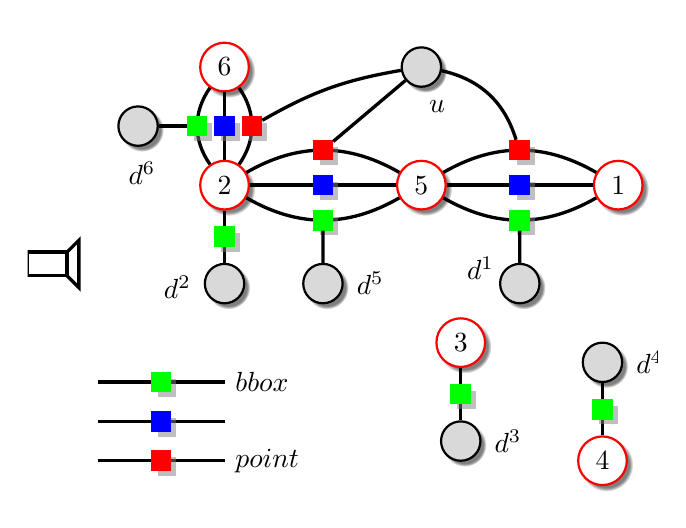
\begin{tikzpicture}[grow cyclic, line width=1.2pt,
    variablenode/.style={circle,circular drop shadow,draw=red,fill=white,thick,minimum width=0.5cm},
   bboxfactor/.style={rectangle,drop shadow,draw=green,fill=green,thick,minimum width=0.2cm},
    collfactor/.style={rectangle,drop shadow,draw=blue,fill=blue,thick,minimum width=0.2cm},
    trackfactor/.style={rectangle,drop shadow,draw=red,fill=red,thick,minimum width=0.2cm},
  obs/.style={fill=gray!30,draw=black},
  prevf/.style={draw=green!20,text=gray},
  prevobsv/.style={draw=gray!10,fill=gray!1,text=gray},
  prevv/.style={draw=red!20,text=gray}
]
  \path[use as bounding box,clip] (-2.5, -5.5) rectangle (5.5,0.5);
  \draw (-2.5,-2.65) rectangle +(0.5,0.3);
  \draw (-2.0,-2.35) -- ++(0.15, 0.15) -- ++(0, -0.6) -- (-2.0, -2.65);
\path
     (0, 0)  node [variablenode] (x6) {6}
++(0, -1.5) node [variablenode] (x2) {2}
++(2.5, 0)  node [variablenode] (x5) {5}
+ (0, 1.5)  node [variablenode,obs] (u) {}
+(.2,1.0)  node {$u$}
+ (.5, -2)   node [variablenode] (x3) {3}
+ (2.3, -3.5)   node [variablenode] (x4) {4}
+(2.5, 0)  node [variablenode] (x1) {1}
;

% Factors between nodes 6 and 2
\draw (x6) edge [bend right=35] node [bboxfactor] (f26) {} (x2);
\path (f26) +(-0.75,0) node [variablenode,obs] (d6) {} 
                        +(-.7,-.6)  node {$d^6$};
\draw (f26) edge (d6);
\draw (x6) edge [bend left=35] node [trackfactor] (ft26) {} (x2);
\draw (ft26) edge [bend left=10] (u);
\draw (x6) edge node [collfactor] {} (x2);

% Factors for node 2
\path (x2) +(0,-1.25) node [variablenode,obs] (d2) {} 
                        +(-.6,-1.3)  node {$d^2$};
\draw (x2) edge node [bboxfactor] {} (d2);

% Factors between nodes 2 and 5
\draw (x2) edge [bend right] node [bboxfactor] (f25) {} (x5);
\draw (x2) edge [bend left] node [trackfactor] (ft25) {} (x5);
\draw (x2) edge [] node [collfactor] {} (x5);
\draw (ft25) edge (u);
\path (x5) ++(-1.25,-1.25) node [variablenode,obs] (d5) {} 
                        +(.6,0)  node {$d^5$};
\draw (f25) edge (d5);

% Factors between nodes 5 and 1
\draw (x5) edge [bend right] node [bboxfactor] (f51) {} (x1);
\draw (x5) edge [bend left] node [trackfactor] (ft51) {} (x1);
\draw (x5) edge [] node [collfactor] {} (x1);
\draw (ft51) edge [bend right] (u);
\path (x1) ++(-1.25,-1.25) node [variablenode,obs] (d1) {} 
                        +(-.5,0.2)  node {$d^1$};
\draw (f51) edge (d1);

% Factors for node 3
\path (x3) ++(0,-1.25) node [variablenode,obs] (d3) {} 
                        +(.6,0)  node {$d^3$};
\draw (x3) edge node [bboxfactor] {} (d3);

% Factors for node 4
\path (x4) ++(0,1.25) node [variablenode,obs] (d4) {} 
                        +(.6,0)  node {$d^4$};
\draw (x4) edge node [bboxfactor] {} (d4);

% Legend
\path (-1.75,-4.0) node (l1s) {} (-0, -4.0) node [anchor=west] (l1e) {$\Energy{bbox}$};
\draw (l1s) edge node [bboxfactor] {} (l1e);
\path (-1.75,-4.5) node (l2s) {} (0, -4.5) node [anchor=west] (l2e) {$\EnergyCol$};
\draw (l2s) edge node [collfactor] {} (l2e);
\path (-1.75,-5.0) node (l3s) {} (0, -5.0) node [anchor=west] (l3e) {$\Energy{point}$};
\draw (l3s) edge node [trackfactor] {} (l3e);

\end{tikzpicture}

    \caption{Graphical model for a single frame with state of car represented
    as single node.  The six numbered nodes represent the unknown state variables of each car. The shaded nodes in the graphical model are observed variables. }
  \label{fig:graphmodel}
\end{figure}

\begin{table}
  \centering
  \begin{tabular}{lrrr}
    \toprule
    Energy & t & yaw & dim \\
    \midrule
    initialization                                                                                  & 3.79 & \textbf{0.86} & 1.64 \\
    $\EnergyLane+\EnergySize+\EnergyBBox+\EnergyDyn                                       $ & 3.83 & 0.90 & \textbf{1.14} \\
    %$\EnergyLane+\EnergySize+\EnergyBBoxocc+\EnergyDyn                                    $ & 3.83 & 0.90 & 1.14 \\
    %$\EnergyLane+\EnergySize+\EnergyBBoxocc+\EnergyDyn+\EnergyCol                         $ & 3.92 & 0.91 & 1.15 \\
    %$\EnergyLane+\EnergyContpttracks+\EnergySize+\EnergyBBoxocc+\EnergyDyn             $ & 3.81 & 0.92 & 1.59 \\
    % \EnergyBBox+\EnergyDyn+\EnergyCol $
    $\EnergyTrackNoOcc+\EnergyCol + \EnergyLane + \dots$  & 3.80 & 0.91 & 1.58 \\
    $\EnergyTrack+\EnergyCol + \EnergyLane + \dots$ & \textbf{3.78} & 0.91 & 1.58 \\
    \bottomrule
  \end{tabular}
  \caption{Localization experiment results with different combination of energies. We report error in three metrics translation error (t) in meters per car, yaw error (yaw) in radians per car and dimension error is again meters per car.}
  \label{tab:localizationExperiment}
\end{table}

% 
% 5. Conclusion and Discussions
% 6. Pacify negative results
\chapter{Discussions}
\section{Conclusions and Future Work}
\label{sec:conclusions}

We have presented a theoretically novel continuous model for occlusion reasoning in 3D. A key advantage is its physical inspiration that lends flexibility towards occlusion reasoning for varied elements of scene understanding, such as point tracks, object detection bounding boxes and detection scores. We demonstrate unified modeling for different applications such as point tracks associations and 3D localization. Our occlusion model can uniformly handle static and dynamic objects, which is an advantage over motion segmentation methods for point-object association. A challenge is that inference for 3D localization is currently slow, requiring a few minutes per window of frames, which prevents exhaustive cross-validation for tuning of weights. Our future work will explore speeding up the inference, for example, by approximating the graph with a tree using the Chow-Liu method \cite{chow1968approximating}, allowing belief propagation for fast inference. Another direction for future work is to replace a single ellipsoid by a set of spheres for modelling a translucent object~\cite{Rhodin2015}, which will better capture object boundary and appearance while remaining a continuous model.



%Our experiments show that our association probability produces more accurate point to object associations when compared to bounding box based association and state of art motion segmentation. Also the localization experiment results show improvement in localization accuracy by modeling occlusions. However, the average translation error of 5 meters is very high. Since the results are averaged over the entire KITTI dataset, there are various possible sources of error, including outliers in point tracks, outliers in detections results.  One of the reasons of poor performance is that we set the parameters $\lambda_{\text{bbox,track,lane,dyn,size}}$ empirically which may be suboptimal. However, because of slow inference algorithms, which take about a day to run on 300 cores for the entire KITTI dataset, learning become infeasible.

%We have several ideas for speeding up inference and thereby allowing learning of weights to become feasible. One of them is to approximate the graph into a tree using Chow-Liu's \cite{chow1968approximating} algorithm and then using Belief Propagation which is linear in the number of edges of the tree.


\chapter{Future Work}

We have come up with model of Object detection energy with occlusion, and our plan is evaluate it
and integrate it with the model.

\section{Object detection energy with occlusion} 

Object detection is usually followed by non-maximal suppression that results in
discarding similar bounding boxes. When we are jointly optimizing detections
with other cues, it is not usually desirable to go with a single bounding box.
Hence, we keep all the bounding box detections by approximating them with
multi-modal sum of Gaussian like logistic functions. We fit the parametric function of the form 
%
\begin{align}
  S(\bb{i}) = \sum_k A_k \exp(-(\bb{i}-\mu^{(d)}_k)^\top \Sigma^{(d)-1}_k
  (\bb{i}-\mu^{(d)}_k))
\end{align}
%
to detection scores, by non-linear error minimization with initialization from
non-maximal suppressed outputs. Here $\mu^{(d)}_j$ is one of the $k$ modes as a
4D vector representing a single bounding box as $[\minx, \miny, \maxx,
\maxy]^\top$. The optimization is constrained with symmetry and positive
definiteness of $\Sigma^{(d)-1}_k$, $\maxx \ge \minx$ and $\maxy \ge \miny$.

\subsection{Detection scores with occlusion reasoning} 
With our model of $\Ptrans$ described in Section \ref{sec:TPmodel}, we can
compute the probability of a point $\mathbf{u}$ on image be occluded assuming
the point is on TP $i$ with mean depth $\mu^{(i)}_d$ as
\begin{align}
  O_{i}(\mathbf{u}, \mu^{(i)}_d) = 1 - \Ptransmud \enspace .
\end{align}

If we know a portion of our proposed detection bounding box is known to be
occluded, then we would like to decrease the confidence in the detection score
about the localization of that end of the object. Assuming that the occlusion
is often on the boundary of detection bounding boxes, we want to decrease our
confidence on the mean detection boundaries around the occluded boundaries.
%One of the simplest ways will be to scale the appropriate diagonal element of
%$\Sigma_j$ by an appropriate scaling factor proportional to occlusion. But this
%does not model explain the affect of occlusion on the non diagonal terms.
%Hence, we choose a covariance addition model where we compute a occlusion
%covariance matrix, that provides a measure of occlusion in each direction.
To re-model our detection scores scaled by continuous occlusion we sample
$O_{i}(\mathbf{u}, \mu^{(i)}_d)$ at the hypothesized detection boundaries from
GMM $S(.)$ and we augment the detection boundary covariance matrix by
$\mathcal{P}_{j} = \rho_{j}\rho_{j}^\top$ where $\rho_{j} = O_{j}(\mathbf{u},
\mu^{(i)}_d)$. The new covariance matrix in detection score is given by 
  $\Sigma'^{(d)}_j = \mathcal{P}_{j} + \Sigma^{(d)}_j$.
%
%\begin{align}
%\end{align}
%
The detection scores GMM with occlusion is given by replacing the covariance
matrix
%
\begin{align}
  S'(\bb{i}) =
  \sum_j A_j \exp(-(\bb{i}-\mu^{(d)}_j)^\top \Sigma'^{(d)-1}_j
  (\bb{i}-\mu^{(d)}_j))
\end{align}

The energy of detection scores is simply take to be the inverse of the detection score.
\begin{align}
  \Energy{detect}(\{ \relp{i}{t} \}_i, \{ \relp{i}{t-1} \}_i, \{\dimsn{i}\}_i ) = \frac{1}{S'(\bb{i})}
\end{align}

\chapter{Appendix}
\label{sec:appendix}
\section{Analytic initialization}
Problem: given detection bounding box and ground plane estimate the unknown parameters i.e. position, orientation and size of the car. This problem is under-determined. Given the bounding box, we just have four constraints while we have six unknowns. To reduce the number of unknowns we assume that detection also gives us an estimate of angle and we assume that length of car is 1.3 times the height. Now, we have 4 unknowns and 4 constraints and we can solve them analytically.

\subsection{Necessary transforms}
Let the ground plane be known with parameters $(\uv{n}, h)$. Let us take the ground plane to be the XY plane with Z axis pointing upwards and origin at the point of intersection of Y-axis with ground plane. The unit vector describing the ground plane is ambiguous by sign, we choose the sign of $\uv{n}$ such that $\hat{n}_2 > 0$, i.e. the unit vector is along the positive Y-axis of the camera based on the assumption that the camera axis are approximately aligned such that Y-axis points downwards and Z-axis to the front.

\begin{align}
  ^gR_c &= [\uv{i}, -\uv{n} \times \uv{i}, -\uv{n}]\\
  ^gt_c &= [0, 0, h]^\top\\
        \text{where} & \\
 \uv{i} &= \frac{1}{\sqrt{\hat{n}^2_3, \hat{n}^2_2}}[0, \hat{n}_3, \hat{n}_2]^\top
\end{align}

In homogeneous coordinates, let the camera to ground transformation be
represented by $^gT_c = \begin{bmatrix}^gR_c & ^gt_c\\ \mathbf{0} &
1\end{bmatrix}$ and its inverse be represented by $^cT_g = {}^gT_c^{-1}$. Let
the yaw of car be given as theta in camera coordinates. Assume it to be same as
ground plane coordinates.

\begin{align}
  \Tr{g}{R}{t} &= \begin{bmatrix}
  \cos(\theta) & \sin(\theta) & 0 \\
 -\sin(\theta) & \cos(\theta) & 0 \\
             0 & 0 & 1
  \end{bmatrix}
\end{align}

\subsection{System of equations}
Let the detected bounding box be represented by $[\xmin, \ymin, \xmax, \ymax]^T$. Let $^cT_t$ be the transformation from tracklet to camera.
\newcommand{\Cu}{C_u}
\newcommand{\Cc}{C_c}
\begin{align}
  \Cu &= \begin{bmatrix}
    0.5 & 0.5 & 0\\
    0.5 & -0.5 & 0\\
    -0.5 & -0.5 & 0\\
    -0.5 & 0.5 & 0\\
    0.5 & 0.5 & 1\\
    0.5 & -0.5 & 1\\
    -0.5 & -0.5 & 1\\
    -0.5 & 0.5 & 1
  \end{bmatrix}\\
  C_i &= \diag( C_{u\{i,:\}} ) \begin{bmatrix}3& 0\\0 & 1 \\1 & 0\end{bmatrix} 
\end{align}

\newcommand{\ttg}{\Tr{g}{\mathbf{t}}{t}}
\newcommand{\tgc}{\Tr{c}{\mathbf{t}}{g}}
\newcommand{\Rgc}{\Tr{c}{R}{g}}
\newcommand{\Rtg}{\Tr{g}{R}{t}}
\newcommand{\Rtc}{\Tr{c}{R}{t}}
\newcommand{\Pgc}{\Tr{c}{P}{g}}
\newcommand{\Ptc}{\Tr{c}{P}{t}}

Consider the projection of i\textsuperscript{th} corner of the car.
\begin{align}
  \lambda_i \mathbf{u}_i &= K(\Rgc(\Rtg C_i[h, w]^\top + \ttg) + \tgc) & \text{ or }\\
  \lambda_i \mathbf{u}_i &= K\Rtc C_i [h, w]^\top + K\Rgc \ttg + K \tgc
  \label{eq:vectorproj}
\end{align}
where $\Rtc = \Rgc\Rtg$, $\ttg = [t_x, t_y, 0]^\top$ is unknown car position in
ground coordinates, $h$ is unknown height, $w$ is unknown width of the car,
$\lambda$ is unknown scale factor and $\mathbf{u}_i$ is the image projection of
i\textsuperscript{th} corner of the car.

Equation \eqref{eq:vectorproj} is a set of 3 equations, the third of which allows us to eliminate $\lambda$ as it gives the $\lambda$ and as a linear combination of $t_x$, $t_y$, $h$ and $w$. Let $\Ptc = K\Rtc$ and $\Pgc = K\Rgc$.
\begin{align}
  \lambda_i \mathbf{u}_i &=  \Ptc C_i [h, w]^\top + \Pgc \ttg + K \tgc\\
  \lambda_i &= \lambda_{hi}  h + \lambda_{wi}  w + \lambda_{tx}  t_x + \lambda_{ty} * t_y + \lambda_c\\
  \text{where} & \\
  \lambda_{hi} &= \Ptc(3, :) C_i(:, 1)\\
  \lambda_{wi} &= \Ptc(3, :) C_i(:, 2)\\
  \lambda_{tx} &= \Pgc(3, 1)\\
  \lambda_{ty} &= \Pgc(3, 2)\\
   \lambda_{c} &= K(3, :) \tgc
\end{align}

\subsection{Approximate solution}
Initial approximate solution can be obtained by assuming that $\ymax$ is the projection either of point 
\begin{align}
  \lambda_c \mathbf{u}_c &= \Ptc[0, 0, \frac{h}{2}]^\top + \Pgc \ttg + K\tgc
\end{align}

Assuming the height to be mean height, we can solve for approximate solution
for $\ttg$. Using this approximate solution find out the corner points that
correspond to the bounding box. Finally \eqref{eq:vectorproj} can be used for
the projected points to solve for exact $[h, w, t_x, t_y]$.

\subsection{Correspondence of bounding box limits to cuboid corners}
The $\xmin$ of bounding can be projection of either of the 8 points of the
cuboid. Once $\xmin$ is chosen the $\xmax$ can be limited to the remain 7
points hence $8 \times 7= 56$ possibilities and similarly $\ymin$ and $\ymax$
lead to 56 different possibilities. In this relatively unconstrained
configuration we have around $56 \times 56 = 3136$ possibilities, which is not
too big but with a little more analysis we can reduce the number. To this
effect we can use the aspect graph of a cuboid to understand the topological
changes by change in view points. Also out of 28 possible configurations in the
aspect graph, we can rule out the configurations that put camera below the
ground plane and directly above the observed car itself. This leaves us with 16
possible topological configurations, which include the symmetrical
configurations when the car is rotated by $180^\circ$. Considering $180^\circ$ symmetry we are only left with 8 possible topological configurations.

A more general way of finding the subset of aspect graph configuration that
need to be configured is to rewrite the bounding box inequalities, 

\begin{align}
  \lambda_i \xmax &\ge \Ptc(1, :) C_i [h, w]^\top + \Pgc(1, :) \ttg + K \tgc\\
  \label{eq:bbox-ineqst}
  \lambda_i \xmin &\le \Ptc(1, :) C_i [h, w]^\top + \Pgc(1, :) \ttg + K \tgc\\
  \lambda_i \ymax &\ge \Ptc(2, :) C_i [h, w]^\top + \Pgc(2, :) \ttg + K \tgc\\
  \lambda_i \ymin &\le \Ptc(2, :) C_i [h, w]^\top + \Pgc(2, :) \ttg + K \tgc \enspace.
  \label{eq:bbox-ineq}
\end{align}
Each of the above four equations is true for all 8 corners, hence there are 32 such inequalities.

The aspect graph boundaries also called the view events, occur when the view
point or the camera optical center crosses the faces of the cuboid object being
viewed. The camera optical center $o_t$ in tracklet coordinate frame is given by.
\begin{align}
  \mathbf{0} &= \Rgc(\Rtg o_t + \ttg) + \tgc\\
  o_t &= -\Rtg^\top \ttg -\Rtg^\top \Rgc^\top \tgc
\end{align}

The 6 faces of a cuboid are simple planes that can be written in terms of $h$
and $g$. A view event occurs whenever we have $o_t$ satisfying equations of any
one of the equations that represent the 6 faces. We have to find the number of
distinct regions that satisfy all of Eq
\eqref{eq:bbox-ineqst}-\eqref{eq:bbox-ineq}. Then for each distinct region we
need to find out the topological configuration that limits the number of
corners candidates for extrema. These can be sorted to create boundaries.


\section{Numerical integration}
Numerical integration is possible by computed by sampling. Samples need to be
generated from the association probability $\assocP$ for a given $j$. We take
proposal distribution to be a GMM with modes around probable reflection points.
The weights of all Gaussians in the mixture are proportional to the distance of
the point $j$ from projection of ellipsoid centre i.e. 
\begin{align}
  A_{ij} = \frac{1}{Z_j}\exp(-(\trackpj{t} - \mu^i_u)^\top\Sigma_u^i(\trackpj{t} - \mu^i_u))
\end{align}
where $Z_j = \sum_{i=1}^N A_{ij}$ and $\mu^i_u$ and $\Sigma_u^i$ are described in \eqref{eq:muiudef} and \eqref{eq:sigmauidef} respectively.
The range of Gaussian $G_i$
must be in the interval $[\|\relp{i}{t}\|, \|\relp{i}{t}\| -
\sqrt{3}\max(\dimsn{i})]$. Hence we take the mean as $\|\relp{i}{t}\| -
\frac{\sqrt{3}}{2}\max(\dimsn{i})$ and variance as
$\frac{1}{3}\max(\dimsn{i})^2$. The distribution from which we sample is 
\begin{align}
  \PropDist(\lambda) = \sum_i A_{ij} \Gauss(\lambda; \|\relp{i}{t}\| -
  \frac{\sqrt{3}}{2}\max(\dimsn{i}), \frac{1}{\sqrt{3}}\max(\dimsn{i}))
\end{align}
And the numerical integral with $K$ samples is computed by
\begin{align}
    \int_1^{\infty}
    \assocP
    \Ereproj(\lambda)
    d\lambda
    =
    \frac{1}{K}\sum_k \Ereproj \frac{\assocPk}{\PropDist(\lambda_k)}
\end{align}
where $\lambda_k$ is the $k$th sample drawn from $\PropDist(\lambda)$.

\section{Sigma of ellipsoid}
\label{sec:sigmacomputation}

\begin{align}
  \muit &= \begin{bmatrix}
  0& 0& \frac{h}{2}
  \end{bmatrix}^\top\\
  \Sigmait &= \begin{bmatrix}
    \frac{4}{l^2} & 0 & 0 \\
    0 & \frac{4}{w^2} & 0 \\
    0 & 0 & \frac{4}{h^2}
  \end{bmatrix}
\end{align}

In tracklet coordinates the equation of ellipsoid is 
\begin{align}
  (\xt - \muit)^\top \Sigmait (\xt - \muit) = 1
\end{align}


Moving to camera coordinates
\begin{align}
  (\Rctot \xc + \tctot - \muit)^\top \Sigmait (\Rctot \xc + \tctot - \muit) = 1
\end{align}

Let $\tcmut = \tctot - \muit$
\begin{align}
  (\Rctot \xc + \tcmut)^\top \Sigmait (\Rctot \xc + \tcmut) = 1
\end{align}
\begin{align}
  \xc^\top \Rctot^\top \Sigmait \Rctot \xc + 2 (\Rctot^\top \tcmut)^\top  \Rctot^\top\Sigmait \Rctot \xc
  + \tcmut^\top \Sigmait \tcmut = 1
\end{align}
Let $\Sigmaic = \Rctot^\top \Sigmait \Rctot$ and $\muic = - \Rctot^\top
\tcmut$
\begin{align}
  (\xc - \muic)^\top\Sigmaic(\xc - \muic) - \muic^\top\Sigmaic\muic +
  \tcmut^\top \Sigmait \tcmut = 1
\end{align}
Let $\Sigmaicf = \frac{\Sigmaic}{1 - \tcmut^\top \Sigmait \tcmut +
\muic^\top\Sigmaic\muic}$
\begin{align}
(\xc - \muic)^\top\Sigmaicf(\xc - \muic) = 1
\end{align}

Hence, we have following expression for mean and sigma of ellipsoid:
\begin{align}
  \label{eq:ellipsoidMeanSigma}
  \muic &= - \Rctot^\top \tcmut \\
  \Sigmaicf &= \frac{\Sigmaic}
{1 - \tcmut^\top \Sigmait \tcmut + \muic^\top\Sigmaic\muic}
\end{align}


\section{Projection of ellipsoid to image}
\newcommand{\mubar}{\bar{\mu}_i}
The perspective projection of an ellipsoid in general is not an ellipsoid in
general. We approximate the projection of ellipsoid by projecting a slice
through the ellipsoid. We choose the slice as the plane perpendicular to the
line joining the center of ellipsoid to the optical center of camera. Let
$\muic$ and $\Sigmaicf$ be the parameters of ellipsoid describing the ellipsoid
in camera coordinates. The any point $x$ on the plane satisfies
$x^\top\frac{\muic}{\|\muic\|} = \|\muic\|$. We introduce 
$\mubar = \frac{\muic}{\|\muic\|^2}$ for notational simplicity. Hence, we want
to project the points that satisfy both the equation of chosen plane and the 
ellipsoid i.e.
\begin{align}
  \mubar^\top x = x^\top\mubar &= 1\\ 
  (x-\muic)^\top\Sigmaicf(x-\muic) &= 1 \enspace.
\end{align}
We rewrite $\muic = \muic\mubar^\top x$, and $1 = x^\top\mubar \mubar^\top x$
\begin{align}
  (x-\muic\mubar^\top x)^\top\Sigmaicf(x-\muic\mubar^\top x) &= x^\top\mubar \mubar^\top x \enspace,
\end{align}
which is equivalent to 
\begin{align}
  x^\top\left((I-\muic\mubar^\top)^\top\Sigmaicf(I-\muic\mubar^\top) - \mubar \mubar^\top\right)x &= 0\enspace.
\end{align}

Note that if $u$ is a projection of $x$ to camera with intrinsic parameters
$K$, then $x = K^{-1}u$ where $u$ is in homgeneous coordinates. Hence the above equation can be re-written as
\newcommand{\Sproj}{\Sigma^{-1}_{\text{proj }i}}
\newcommand{\Sperpcut}{\Sigma^{-1}_{\text{perpcut }i}}
\begin{align}
  u^\top\Sproj u &= 0\enspace, 
\end{align}
where $\Sproj = K^{-\top}\Sperpcut K^{-1}$ and 
\begin{align}
  \Sperpcut = (I-\muic\mubar^\top)^\top\Sigmaicf(I-\muic\mubar^\top) - \mubar \mubar^\top \enspace.
\end{align}

\begin{comment}
  \section{Bounding box energy}
  \label{sec:totalBBoxEnergy}
  With abuse of notation we represent the four sides of hypothesized bounding
  box by $\projectionOf{\dimsn{i}}$ and detected bounding box by $\bb{i}$.
  Suppose the bounding box $i$ is occluded by bounding box $i$ then the
  bounding box energy becomes a pairwise term.

  \begin{multline}
    \pEnergy{occ}(\relp{i}{t}, \dimsn{i}, \relp{j}{t}, \dimsn{j}) = \\
    \sum_s \rho^{ijs}(t)\projectionOf{\dimsn{i}}_s - \bb{i}_s
               %\sum_{i=1}^N \sum_{t=s_i}^{e_i}
    %\sum_kp_{ik}^{\text{track}}(\projectionOf{\dimsn{i}} - \bb{k})^\top \pmb{\rho}(i,j,t)
  \end{multline}
  where $\rho^{ijs}(t)$ is the visibility fraction of the side $s$ of the
  bounding box. We need to compute visibility fraction we need to compute the
  occlusion mask which is explained in next few sections.

  \subsection{Visible faces from bounding boxes}

  \begin{figure}[h]
    \includegraphics[width=\columnwidth]{graphics/maxFacesVisible.pdf}
    \caption{Only three faces can be visible out of six faces of a bounding
    box.}
  \end{figure}

  Each bounding box has 6 faces of which only 3 can be visible.
  Sort the vertices in increasing order of depth. The closest vertex has three
  neighboring faces. All the faces that are visible must be a subset of these
  three. Use first three vertices to
  define the front face (say $\frontface$). Also identify the four 3D points
  that correspond to min/max in x and y direction in the image. If all min-max 4
  points are same as vertices of $\frontface$, then we have only one plane
  visible. If $\{\minx, \maxx\} \not\subset \frontface \land \{\miny, \maxy\}
  \not\subset \frontface$ then we have 3 planes visible. Otherwise we have just
  two planes visible. Let number of planes visible be $n_F$.

  \begin{align}
    n_F &= \begin{cases}
    1 & \text{if }\{\minx, \maxx, \miny, \maxy\} =
    \frontface\\
    2 & \text{else if }\{x_{\text{min}}, x_{\text{max}}\} \subset \frontface \lor
    \{y_{\text{min}}, y_{\text{max}}\} \subset \frontface
    \\
    3 & \text{else if }\{x_{\text{min}}, x_{\text{max}}\} \not\subset \frontface \land
    \{y_{\text{min}}, y_{\text{max}}\} \not\subset \frontface
    \end{cases}
    \label{eq:nfaces}
  \end{align}

  First vertex restrict possible visible faces to three faces. If $n_F = 3$,
  then all three of these faces are visible. If $n_F = 2$, use second closest
  vertex to restrict visible faces to just two. If $n_F = 3$, then front face 
  $\frontface$ is the only visible face.
\end{comment}

\begin{comment}
  \subsection{Occlusion mask}
  % Initialize empty mask polygon $\occ{0}$ at depth $d=0$.
  % \begin{itemize}
  %   \item Sort all cars in increasing order of depth
  %   \item for each car $i$ in the sorted list
  %     \begin{itemize}
  %       \item Update mask polygon: \\
  %         $\occ{\relpz{i}{t}} = \occ{d} \cup \projectionOf{\dimsn{i}}$
  %       \item $d = \relpz{i}{t}$
  %     \end{itemize}
  % \end{itemize}

  % Sort all planes in increasing order of depth.  This yields a cumulative
  % occlusion mask function
  Occlusion mask is a function that takes the relative depth $d$ from the car
  camera and returns a binary mask that represents occlusions untill that depth.
  Near to the camera occlusion mask is all empty (all zeros) and more occlusions
  get added to the mask with distance.

  \begin{align}
    \occ{d} &= \begin{cases}
    \phi & \text{if } 0 < d \le \relpz{1}{t}\\
    \cup_{i=1}^j \projectionOf{F^i} & \text{if } \relpz{1}{t} < d \le \relpz{j+1}{t}
    \end{cases}
    \label{eq:occlusionmask}
  \end{align}

  where $\relpz{j}{t}$ is the depth of the $j$th TPs participant when sorted
  by increasing depth.

  \subsection{Algorithm to get faces based occlusion mask}
  \label{sec:occlusionMaskFromOptVector}

  This is an algorithm to compute occlusion mask Eq.\eqref{eq:occlusionmask}. We
  represent the occlusion mask as a set of polygons.

  Initialize empty mask polygon $\occ{0}$ at depth $d=0$.
  \begin{enumerate}
    \item Collect visible faces using Eq.\eqref{eq:nfaces} for all cars
    %\item for each face get its closest and farthest vertex to the camera.
    \item Create a sorted list of faces
    % \item Create a sorted binary tree of
    %   faces indexed by closed vertices.
    \item Loop over list of sorted visible faces
      \begin{enumerate}
        \item Get the face(s) $\{\face\}$ closer to camera than this face
        \item Add the faces to mask polygon (if not already added): \\
          $\occ{\relpz{i}{t}} = \occ{d} \cup \projectionOf{\face}$
        \item $d = \relpz{i}{t}$
      \end{enumerate}
  \end{enumerate}

  To get the occlusion mask for a face use the farthest vertex of the face to
  query $\occ{.}$.

  \subsection{Visibility fraction of a side}
  Let the center of the projected hypothesized bounding box be $\centerProj$ and
  the four corners be $\{\cornerProj{k}\}_{k=1}^{4}$ . Each side and the center
  of the bounding box form a triangle, for example $\triangleProj{1,2} =
  \{\cornerProj{1}, \cornerProj{2}, \centerProj\}$. We take the visibility of
  this triangle as a visibility of the side $s = (1,2)$. Hence the visibility
  fraction of side is given by
  \begin{align}
    \rho^{ijs}(t) = \frac{\|\triangleProj{s} \setminus \occ{\relpz{i}{t}}\|}
                         {\|\triangleProj{s}\|}
     \label{eq:bboxEnergyFromOccMask}
  \end{align}
\end{comment}

\begin{comment}
  \section{Occlusion free projection}
  Occlusion free projection can be obtained by applying the precomputed occlusion
  mask to the face projection.
  \begin{align}
    \occFreeProj{\face} &= \projectionOf{\face} \setminus
    \occ{\relpz{i}{t}}
  \end{align}

  \section{Perspective-visibility fraction}

  Apart from occlusion, we want to account for the perspective affects. When an 
  objects perspective projection is too small, detection and all related
  evidences deteriorate. One way of this is to find out the projection ratio. In
  fact, we can consolidate projection ratio and occlusion ratio in one term if
  we consider the projection of 3D bounding box planes instead of the entire
  bounding box. 

  \begin{align}
    \rho^i_t &= \sum_{k=1}^{n_F}\frac{\relpz{i}{t}^2\|\occFreeProj{F^i_k(t)}\|}{f^2\|F^i_k(t)\|}
  \end{align}

  where $\occFreeProj{.}$ again means occlusion free projection. $f$ is the
  focal length of the camera so that $\frac{f^2}{\relpz{i}{t}^2}\|F^i_k(t)\|$ is
  the area of projected plane if there were no perspective effects.
\end{comment}


\begin{comment}
  
\begin{table*}
  \begin{tabular}{|l|r|r|l|}
    \hline
    func            & equation                      & ms per 6 frames &
    comment \\
    \hline
    totalBBoxEnergy & Sec \ref{sec:totalBBoxEnergy} & 268 & \\
    laneEnergy      & Sec \ref{sec:laneEnergy}      & 163 & \\
    laneOrientationEnergy & Eq \eqref{eq:laneOrientationEnergy} & 155 & The
    equation summed up for all 6 tracklets\\
    collisionEnergyHellingerDistance & Eq 
    \eqref{eq:collisionEnergyHellingerDistance} & 93  & \\
    totalPosTransitionEnergy & Eq \eqref{eq:totalPosTransitionEnergy} & 15 & \\
    totalSizeEnergy & Eq \eqref{eq:totalSizeEnergy} & 0.9 & \\

    \hline
    occlusionMaskFromOptVector & Sec \ref{sec:occlusionMaskFromOptVector} &
    123 &
    \\
    bboxEnergyFromOccMask & Eq \eqref{eq:bboxEnergyFromOccMask} & 140 &  \\
    vis\_area\_from\_triangle & $\|\triangleProj{s} \setminus
    \occ{\relpz{i}{t}}\|$ & 76 & \\
    \hline
    distance2curve & $\text{DIST}(L_j(k), x)$ & 74 & Called 2 times per
    tracklet \\
    filterMapWaysByDistance & $M_{\text{close}} = \{m : \text{DIST}(.) < 50\} $ & 52 & \\
    area\_of\_triangle & $\|\triangleProj{s}\|$ & 48 & called 4 times per
    tracklet \\
    occlusionMask & Step 3 of Sec \ref{sec:occlusionMaskFromOptVector} & 46 &
    \\
    \hline
  \end{tabular}

  \begin{tabular}{|l|r|r|l|}
    \hline
    func            & equation                      & ms per 6 frames &
    comment \\
    \hline
    totalContPtTracksEnergy & Sec \ref{sec:totalContPtTracksEnergy} & 25000 &
    \\
    integrand & Eq \eqref{eq:integrand} & 23000 & \\
    repmat & & 5000 & \\
    assocCoeffEval & Eq \eqref{eq:assocCoeffEval} & 4000 & \\
    evalPreflection & Eq \eqref{eq:analytic-prefl} & 3000 & \\
    gradfocci & $\nabla \occf^\top \ray$ & 2040 & \\
    associationCoefficientInit & Eq
    \eqref{eq:ptransmissionInit}\eqref{eq:ellipsoidMeanSigma} & 1706 & \\
    projectToImage & $\frac{Ku}{Ku(3)}$ & 4000 & Called ~8 times per edge\\
    evalCumulativePtrans & \eqref{eq:evalCumulativePtrans} & 1178 & \\
    ptransmissionApproxInit & \eqref{eq:ptransmissionInit} & 1000 & \\
    ellipsoidCentreDist & $(x-\mu)^\top \Sigma (x-\mu)$ & 1000 & \\
    squeeze & & 951 &\\
    trackletToCamTransform & $R_{\ori{i}{t}}, t$ & 786 & \\
    ellipsoidMeanSigma & Eq \eqref{eq:ellipsoidMeanSigma} & 812 & \\
    \hline
  \end{tabular}
\end{table*}

\end{comment}

\begin{comment}%%%%%%%%%%%%% May or may not use %%%%%%%%%%%
TODO: Write Introduction
  NEC has already developed a monocular camera based structure from motion
  system which is accurate for requirements of road scene understanding. So we
  assume that egomotion is given as an observed variable in our graphical
  model. And we have following features to our disposal for estimating the 3D
  poses (position + orientation) of traffic participants (TPs):
  \begin{description}
    \item[Ground plane] We assume that all the TPs lie on a common ground
      plane. This is not particularly true for the cars that are parked off the
      road. However, for autonomous driver assistance applications we can
      ignore those cars.
    \item[Detections] We assume that 2D car detections are available with tracking informations.
    \item[Point tracks] We assume that 2D point tracks are available.
    \item[GPS and Map information] We assume that GPS information is available
      and we use openstreetmaps.org for pulling out local map for the current
      car's position.
    \item[Lane Information] We assume the lane detection works well and lane
      information is available.
    \item[Size prior] The distribution of size of cars follows gaussian distribution.
    \item[Collision] A reasonable output of the system donot has any overlapping cars.
  \end{description}
\end{comment}

  \section{Uncertainty addition in measurement}
  Consider that we have a set of measurements whose mean and variance are known $\mu = E(x)$ and $\Sigma = E ((x - \mu_x)(x - \mu_x)^\top)$. We want to know the
  affect of uncertainty on mean and variance of existing observations. On adding
  noise $[\Delta x, \Delta y]^\top$ with zero mean and covariance $\Delta
  \Sigma = E(\Delta x \Delta x^\top)$ the covariance of new data is given by
  \begin{align}
    E((x + \Delta x)(x+\Delta x)^\top) = E(xx^\top) + E(x \Delta x^\top) %\\
    + E(\Delta x x^\top) + E(\Delta x \Delta x^\top)
  \end{align}
  where the terms $E(x \Delta x^\top)$ denote the correlation between the data
  vector and the uncertainty in the data. Although we understand that in our case
  the data is the appearance based detection score and uncertainty because of
  occlusion is closely related to the appearance and hence detection score, we
  assume independence between $x$ and $\Delta x$. Hence our resultant covariance
  matrix $ E((x + \Delta x)(x+\Delta x)^\top) = \Sigma + \Delta \Sigma$
  are 4D. But that should not be a problem because the detection scores are
  modeled as $[x_{\text{min}}, y_{\text{min}}, x_{\text{max}},
  y_{\text{max}}]^\top$, we can stack the vectors in the soft occlusion region
  domain as the regions are independent of min or max variation. The parameters
  of 4D occlusion distribution are given by

  \begin{align}
    \mu'_{Oij} = [\mu_{Oij}^\top \mu_{Oij}^\top]^\top
    \Sigma'_{Oij} = \begin{bmatrix}
      \Sigma_{Oij} & \Sigma_{Oij} \\
  \Sigma_{Oij} & \Sigma_{Oij}
    \end{bmatrix}
  \end{align}

  With our
  discussion so far, the function $O_{ij}(.)$ gives an additional measure of
  uncertainty associated with each point in the space.

% Explanation of Beizer curves is not needed %%%%%%%%%%%%%%%%%%%
% A lane is modeled by four control points of a \Beizer curve $L_j = \{l_0, l_1,
% l_2, l_3\}$. The parametric curve is given by $L_j(k) = \sum_{i=0}^3 {}^3C_i
% (1-t)^{3-i}t^i l_i$. \Beizer are double differentiable so one can find
% tangents ($L'_j(k)$) and normals $R_{\frac{\pi}{2}}L'_j(k)$ where 
% $R_{\frac{\pi}{2}} = \begin{bmatrix} 0 & -1 \\ 1 & 0 \end{bmatrix}$ is
% $90^\circ$ rotation matrix.

%Using standard algorithms \cite{ma2003point, chen2007improved}, we 
%approximate the closest point on a \Beizer curve $k_x = \projOnLane{x}$.
%Consequently one can get solutions for shortest distance $s =
%\text{DIST}(L_j(k), x)$ and orientation at a closest point on the lane
%$\mathbf{t} = \text{TAN}(L_j(k), x)$.

% \subsection{Position in lane}
%
% \begin{align}
%   \Energy{plane} &=
%   \min_{j = 0}^{n_l} \text{DIST}(L_j(k), \pos{i}{t})
% \end{align}
%
 % 
 % We normalize it with the confidence in lane positions.
 % 
 % \begin{align}
 %   \Energy{plane} &=
 %   \min_{m = 0}^{n_l} \text{DIST}(L_m(k), \pos{i}{t})
 %   \LaneUncertainty{\pos{i}{t}}
 % \end{align}



%\subsection{Orientation within lane}
%\begin{itemize}
%\end{itemize}

% \begin{align}
%   \Energy{olane} &= 1 - \text{TAN}(L_l(k),  \pos{i}{t})
%   \cdot
%   \ori{i}{t}
% \end{align}
% 
% 
% 
% This model needs to be scaled by uncertainty. For example, if we want to say
% that the farther the lane is from the camera we are less sure about lane
% orientation and hence this evidence term we scale it by say square of distance
% of the car position from camera.

% \begin{align}
%   \Energy{olane} &= 
%   (1 - \ori{i}{t} \cdot \text{TAN}(L_{m^*}(k),  \pos{i}{t}) )
%   
% \end{align}
% where $m^* = \arg \min_m \text{DIST}(L_m(k), \pos{i}{t})$



\begin{comment}
    
\section{Collisions}

The collision constraint among TPs can be modelled by
pairwise distance based constraints. But having constraints between each pair
of participants is bound to create cycles and computational inefficient.
Among game developers it is common to use spatial hashing to find collision
candidates and use pairwise constraints only among those. While this will
enable us to speed up collision checking, we will still end up inducing cycles
in the model. There are two ways to break these cycles, 1) disable the cross
lane collision checking 2) created a weighted graph among collision
candidates weighted by distance and then find a minimum spanning
tree to break cycles. (1) is too strong of an assumption hence we focus on the
second approach.

There are two possible approaches to find collision among candidates (1)
polygon intersection methods (2) soft ellipse intersection method. Boost
provides scan line based approach to find intersections of polygons. Since our
polygons are simple rectangles, this approach can be very fast. Other approach
is to approximate rectangles with ellipses and finding if the ellipses
intersect.  This intersection can be computed analytically.

\begin{align}
  \EnergyCol &= \begin{cases}
  \infty &\text{if INTERSECTS}(\pos{i}{t}, \dimsn{i}, \pos{j}{t},
  \dimsn{j})\\
  0 &\text{otherwise}
  \end{cases}
\end{align}

%For smoother collision probability see Section \ref{sec:smoothercollision}.


\subsection{Ellipse-ellipse intersection}
\label{sec:ellipseintersection}
A rectangle with sides $2a$ and $2b$ can be approximated by an ellipse with
equation $\frac{x^2}{a^2} + \frac{y^2}{b^2} = 1$. But this ellipse is inside
the rectangle. To enclose the rectangle, scale the ellipse by a factor of
$\sqrt{2}$. The equation becomes, $\frac{x^2}{2a^2} + \frac{y^2}{2b^2} = 1$.
For rotation $\psi$ and center $\pos{i}{t}$, the equation of ellipse can be
re-written as:
\begin{align}
  (\mathbf{x} - \pos{i}{t})^\top\Sigma_i^{-1}(\mathbf{x} - \pos{i}{t}) &= 1
\end{align}
where
\begin{align}
  \Sigma_i^{-1} &= \begin{bmatrix}
    \frac{\cos^2{\psi}}{2a^2} + \frac{\sin^2{\psi}}{2b^2} &
    \frac{\cos{\psi}\sin{\psi}}{2}(\frac{1}{b^2} - \frac{1}{a^2})\\
    \frac{\cos{\psi}\sin{\psi}}{2}(\frac{1}{b^2} - \frac{1}{a^2}) &
    \frac{\sin^2{\psi}}{2a^2} + \frac{\cos^2{\psi}}{2b^2} \\
  \end{bmatrix}
\end{align}

% A point $\mathbf{x}$ is inside both ellipse $i$, $j$ if and only if
% \begin{multline}
%   (\mathbf{x} - \pos{i}{t})^\top\Sigma_i^{-1}(\mathbf{x} - \pos{i}{t}) +\\
% (\mathbf{x} - \pos{j}{t})^\top\Sigma_j^{-1}(\mathbf{x} - \pos{j}{t})
%   \le 2
% \end{multline}
% which is equivalent to
% \begin{multline}
%   (\mathbf{x} - \mu_c)^\top\Sigma_c^{-1}(\mathbf{x} - \mu_c)
%   + \pos{i}{t}^\top\Sigma_i^{-1}\pos{i}{t}\\
%   + \pos{j}{t}^\top\Sigma_j^{-1}\pos{j}{t}
%   - \mu_c^\top\Sigma_c^{-1}\mu_c
%   \le 2
% \end{multline}
% where $\Sigma_c = (\Sigma_i^{-1} + \Sigma_j^{-1})^{-1}$ and $\mu_c =
% \Sigma_c(\Sigma_i^{-1}\pos{i}{t} + \Sigma_j^{-1}\pos{j}{t})$.
% 
% There is at least one point inside both ellipse if 
% \begin{align}
%   \pos{i}{t}^\top\Sigma_i^{-1}\pos{i}{t}
%   + \pos{j}{t}^\top\Sigma_j^{-1}\pos{j}{t}
%   - \mu_c^\top\Sigma_c^{-1}\mu_c
%   &\le 2
% \end{align}
% 
% The left hand side can be interpreted as distance between two ellipses, which
% is 2 when the two ellipses collide and $0$ when two ellipse completely
% overlap.

\subsection{Smoother collision probability}
\label{sec:smoothercollision}
%The above mentioned ellipse-ellipse intersection formulation gives us an
%insight: the distance between two oriented ellipse boundaries can be again
%formulated as a distance metric\footnote{TODO:proof}.
Instead of using Gaussians to model
collision constraints as done by \cite{milan2013continuous}, we use a more
steeper sigmoid function.
\begin{multline}
  \EnergyCol = \frac{1}{1 +
\exp(-k(\pos{i}{t}^\top\Sigma_i^{-1}\pos{i}{t})-1)}\\
\frac{1}{1 +
\exp(-k(\pos{j}{t}^\top\Sigma_j^{-1}\pos{j}{t})-1)}
\end{multline}
where $k$ is steepness parameter.
%$d(.)$ is the distance metric defined as:
%\begin{multline}
%  d(\pos{i}{t}, \dimsn{i}, \pos{j}{t}, \dimsn{j})
%  =
%  \pos{i}{t}^\top\Sigma_i^{-1}\pos{i}{t} \\
%  + \pos{j}{t}^\top\Sigma_j^{-1}\pos{j}{t}
%  - \mu_c^\top\Sigma_c^{-1}\mu_c
%\end{multline}

\end{comment}



\begin{comment}
\section{Analytical attempt to integration}
  %%%%%%%%%%%%%%%% Analytical attempt to integration %%%%%%%%%%%%%%%%%%%%%
  \begin{align}
    E^i_{\text{reproj}}(\lambda) &= \left\|\trackpj{t} - \frac{p_{1:2}\lambda +
  q_{1:2}}{p_3\lambda + q_3}\right\|^2\\
  &= \frac{(p_1\lambda + q_1 - u_{j1}(t))^2 + (p_2\lambda + q_2 - u_{j2}(t))^2}
  {(p_3\lambda + q_3)^2}\\
  &= \frac{a\lambda^2 + b\lambda + c}{(p_3\lambda + q_3)^2}
  \end{align}
  where $a = p_1^2 + p_2^2$, $b = 2p_1(q_1 - u_{j1}(t)) + 2p_2(q_2 - u_{j2}(t))$
  and $c = (q_1 - u_{j1}(t))^2 + (q_2 - u_{j2}(t))^2$

  So, in terms of $\lambda$ we have the integrand as
  \begin{multline}
    \int_1^\infty
    \prod_i (1 +
    \tanh(\poly^{(1)}_{ij1}(\lambda)))\sech^4(\poly^{(2)}_{ij2}(\lambda))\\
    (\max\{ 0, \poly^{(2)}_{ij3}(\lambda) \})^2
    \frac{\poly^{(2)}_{ij4}(\lambda)}{(\poly^{(1)}_{ij5}(\lambda))^2}d\lambda
  \end{multline}
  where $\poly^{(n)}_{ijk}$ denotes a polynomial $k$ of order $n$ dependent upon $i$th
  TP and $j$th point. This integrand is still too difficult to
  be solved or approximated analytically.

  We approximate the expression,

  \begin{multline}
    \prod_i \Llambda
  \sech^4\left(\frac{k}{2}\dishort\right)(\max\{ 0, \nabla k\dishort^\top\ray \})^2
  \end{multline}

  with a
  gaussian with mean at $\mu^{ij}_{\lambda} : d_i(\mu^{ij}_{\lambda}\ray) = 0$
  standard deviation as $\sigma^{ij}_{\lambda} =
  \frac{\pi}{2\sqrt{3}kd(\mu^{ij}_{\lambda}\ray, \pos{i}{t-1})}$  and magnitude as the
  expression computed at mean. An integrand of the form
  \begin{align}
    \frac{\poly^{(2)}_{ij4}(\lambda)}{(\poly^{(1)}_{ij5})^2}
      e^{\frac{- (\lambda -
  \mu^{ij}_{\lambda})^2}{\sigma^{ij}_{\lambda}}}
  \end{align}
   is integrable analytically by parts.

   \begin{align}
   \int_1^\infty \frac{a\lambda^2 + b\lambda + c}{(p_3\lambda + q_3)^2}e^{\frac{- (\lambda -
  \mu^{ij}_{\lambda})^2}{\sigma^{ij}_{\lambda}}}d\lambda
   \end{align}
   Substituting $y = \frac{\lambda - \mu^{ij}_{\lambda}}{\sigma^{ij}_{\lambda}}$

   \begin{align}
     \int_1^\infty \frac{a_y y^2 + b_yy + c_y}
     {(p_{3y}y + q_{3y})^2}e^{-y^2}dy
   \end{align}
   where $a_y = a(\sigmaijl)^3$, $b_y = (2a\muijl + b)(\sigmaijl)^2$ and $c_y =
   (2a(\muijl)^2 + b\muijl + c)\sigmaijl$ and $p_{3y} = \sigmaijl p_3$ and
   $q_{3y} = p_3\muijl + q_3$
  
\end{comment}


  % \subsection{Sandwich of ellipsoids model}
  % 
  % \begin{enumerate}
  %   \item Model $\occf$ as
  %     sigmoid over ellipse instead of a gaussian.
  %     \begin{align}
  %       \occf = \frac{1}{
  %       1 + e^{-(\mathbf{x} - \pos{i}{t})^\top
  %         \Sigma_i (\mathbf{x} - \pos{i}{t}))}}
  %     \end{align}
  %   \item To get the intuition of this occupancy function imagine the traffic
  %     participant as layered ellipsoid. The innermost ellipsoid has very high
  %     probability (approx 1) of being occupied. The outermost ellipsoid has very
  %     low probability (approx 0) of being occupied. We will just consider the
  %     occupancy interplay within these two ellipsoids.
  %   \item Project outer ellipsoids of all TP's on the image.
  %   \item Consider the ellipses that bound the track point $\trackpj{t-1}$.
  %   \item For each ellipse do
  %     \begin{itemize}
  %       \item Case 1: The ray intersects inner ellipse
  %         Now the ray intersects both inner and outer ellipse
  %         Compute the intersection points on both the ellipses
  %         Compute the gradient function $\nabla\occf^\top \ray$ at
  %         the mid point of the two intersections. Use this as the magnitude of
  %         gaussian mixture component centered at the mid point of intersections
  %         and spread such that 97 percentile of probability mass of guassian is
  %         within the intersection points. With the same parameters model the
  %         transimission probability with product of logistic function $L(.)$.
  %       \item Case 2: The ray do not intersects inner ellipse.
  %         The ray just passes through the outer ellipse. Find the point on the
  %         ray closest to the center of the ellipse. Compute gradient function
  %         at the closest point, which will be again used as the magnitude of
  %         gaussian mixture component centered at the closest point and spread
  %         such that 97 percentile of probabiltiy mass of gaussian is within the
  %         two intersection points of the ellipse. With the same parameters model
  %         the transimission probability with product of sigmoids.
  %     \end{itemize}
  %   \item Now this approximated $\lambdadist = \sum N(.) \prod (1 - L(.))$ can
  %     be used in integrating the error over $\lambda$.
  % \end{enumerate}
  \newpage

  \clearpage
  %%%%%%%%%%%%%%%% Analytical attempt to integration %%%%%%%%%%%%%%%%%%%%%

% \section{Object detection score}
% \begin{align}
% \Energy{det}(\relp{i}{t}, \dimsn{i}) = 
%              \frac{1}{S_t^2(\projectionOf{\dimsn{i}})}
% \end{align}

% \section{Object 2D bounding box with occlusion}
% Reproduced from \cite{song2014eccv} section 4.3
% 
% \begin{multline}
%   \Energy{box}(\relp{i}{t}, \dimsn{i}) =
%              %\sum_{i=1}^N \sum_{t=s_i}^{e_i}
%              \rho^i_t \|\projectionOf{\dimsn{i}} -
%              \bb{i}\|^2
% \end{multline}
% 
% where $S_t(.)$ is the function to approximate the detection scores using
% mixture of Gaussian model and $\rho^i_t$ is the visibility fraction. 
% 
% % It can be
% % computed by using polygon intersection algorithms.
% % \begin{align}
% %   v^i_t &= \frac{\|\occFreeProj{\dimsn{i}}\|}
% %                 {\|\projectionOf{\dimsn{i}}\|}
% % \end{align}
% % where $\|.\|$ represents the norm or the area of the polygon.
% 
% Another approach is to just consider the corner points in the occlusion free
% area.  Say $\projectionOf{\dimsn{i}} = [b^i_1, \dots, b^i_4]$.
% \begin{multline}
%   \Energy{box}(\relp{i}{t}, \dimsn{i}) =
%              %\sum_{i=1}^N \sum_{t=s_i}^{e_i}
%              %S_t^2(\projectionOf{\dimsn{i}})
%              \sum_{{b^i_j} \in \occFreeProj{\dimsn{i}}}
%              \|b^i_j - d^i_j\|^2
% \end{multline}
% 
% In the opinion of this author, the second approach is better because the
% visibility is an area based measure while the error metric is point to point
% distance based measure. If we use bounding overlap instead of corner to corner
% distance, the use of visibility fraction makes much more sense. However, one
% can argue that even detection score is an area based measure. 
% 
% Hence a third approach can be 
% \begin{multline}
%   \Energy{box}(\relp{i}{t}, \dimsn{i}) =
%              %\sum_{i=1}^N \sum_{t=s_i}^{e_i}
%   \rho^i_t \|\projectionOf{\dimsn{i}} \ominus \bb{i}\|
% \end{multline}
% where $A \ominus B$ represents the symmetric difference between set $A$ and set
% $B$ and is given by $A \ominus B = (A \cup B) \setminus (A \cap B)$.
% One may argue that we can take the intersection of occlusion free projection 
% and get rid of the visibility fraction, but that would be a little off the 
% detection bounding box is usually more close to the projection of full car
% instead of the just the visible portion.
% 
% 
% \section{Orientation cues}
% There are two orientation cues (1) orientation from detection (2) orientation
% from appearance map \cite{yao2012describing}.
% 
% \begin{align}
%   \Energy{ori} &= 
%   %S_t^2(\projectionOf{\dimsn{i}})
%   \rho^i_t(1 - \cos({\omega}^i_{\text{det}} - \ori{i}{t})
% \end{align}
% 
% Appearance map is a shape prior that requires \emph{Scene labeling} input.


{\small
  \bibliographystyle{ieee}
  \bibliography{continuousocclusion}
}
\end{document}

  
